\section{Modules}

\subsection{STimers}
There are several situations where the application doesn't need such hard real-time precision for timing actions and we just need that a section of code will execute when at least, some amount of time has elapsed. For these purposes, STimers (Software-Timers) is the right module to use. 

The STimers implementation doesn't access resources from the interrupt context, does not consume any significant processing time unless a timer has actually expired, does not add any processing overhead to the \textit{sys-tick} interrupt, and does not walk any other data structures. The timer service just takes the value of the existing kernel clock source for reference ($\ t_{sys}$ ), allowing timer functionality to be added to an application with minimal impact.

\begin{figure}[H]
    \centering
    \begin{tikzpicture}[every node/.style= {font=\scriptsize, text height=1ex, text depth=.25ex,},scale=1.5]
        \draw[->] (0,0) -- (8.5,0);
        \foreach \x in {0,1,...,8}{
            \draw (\x cm,3pt) -- (\x cm,0pt);
        }
        \node[anchor=north] at (1,0) {$t_0$};
        \node[anchor=north] at (1,-0.2) {armed};
        \node[anchor=north] at (2,0) {...};
        \node[anchor=north] at (3,0) {$t-2$};
        \node[anchor=north] at (4,0) {$t-1$};
        \node[anchor=north] at (5,0) {$t$};
        \node[anchor=north] at (6,0) {};
        \node[anchor=north] at (8.5,0) {$\ t_{sys}$ (tick)};
        \fill[myLightGray] (1,0.25) rectangle (2,0.4);
        \fill[myDarkGray] (2,0.25) rectangle (3,0.4);
        \fill[myMoreDarkRed] (3,0.25) rectangle (4,0.4);
        \fill[myDeepGray] (4,0.25) rectangle (5,0.4);
        \draw[myDeepGray,dashed,thick,-latex] (5.05,0.325) -- (6.05,0.325);
        \draw[decorate,decoration={brace,amplitude=5pt}] (1,0.45) -- (5,0.45) node[anchor=south,midway,above=4pt] {elapsed $\ E_t$};
        \draw[myDeepGray,thick,-latex] (1,1) -- (1, 0.5 ) node[anchor=north,midway,below=1pt] {};
        \draw[myDeepGray,thick,-latex] (5,-0.7) -- (5, -0.3 ) node[anchor=north,midway,below=1pt] {};
        \draw[myDeepGray,thick,-latex] (1,-1) -- (1, -0.5 ) node[anchor=north,midway,below=1pt] {};
        \node[anchor=north, font=\ttfamily] at (1,1.4) {\tiny qSTimerSet(\&X, Et)};
        \node[anchor=north] at (8.5,0) {$\ t_{sys}$ (tick)};
        \node[anchor=north] at (1,-1.2) {$\ \left.X\right\vert_{ti=t_0}^{T_X=E_t}$};
        \node[anchor=north] at (5,-0.7) {$\ X$ expiration};
        \node[anchor=north] at (5,-1.2) {$\ \left ( t_{sys} - X_{t_i} \right ) \geq X_{T_X}$};
    \end{tikzpicture}
    \caption{STimers operation}
    \label{fig:stimers}
\end{figure}

As illustrated in figure \ref{fig:stimers}, the time expiration check is roll-over safe by restricting it, to the only calculation that make sense for timestamps, $\ t_{sys} - X_{T_x}$, that yields a duration namely the amount of time elapsed between the current instant($\ t_{sys}$ ) and the later instant, specifically, the tick taken at the arming instant with \lstinline{(qSTimer_Set())}, ($\ X_{t_i}$ ).
Thanks to modular arithmetic, both of these are guaranteed to work fine across the clock-source rollover(a 32bit unsigned-counter), at least, as long the delays involved are shorter than 49.7 days. 
\medskip

\textbf{Features:}
\begin{itemize}
    \item Provides a non-blocking equivalent to delay function.
    \item Each STimer encapsulates its own expiration (timeout) time.
    \item Provides elapsed and remaining time APIs.
    \item As mentioned before, STimers uses the same kernel clock source, this means the time-elapsed calculation use the \lstinline{qClock_GetTick()} API, therefore, the time resolution has the same value passed when the scheduler has been initialized with \lstinline{qOS_Setup()}.
\end{itemize}

\subsubsection{Using a STimer}
A STimer is referenced by a handle, a variable of type \lstinline{qSTimer_t} \index{\lstinline{qSTimer_t}} and preferably, should be initialized by the \lstinline{QSTIMER_INITIALIZER} constant before any usage. 

To use them, the code should follow a specific pattern that deals with the states of this object. All related APIs are designed to be non-blocking, this means there are ideal for use in cooperative environments as the one provided by the OS itself. To minimize the implementation, this object is intentionally created to behave like a binary object, this implies that it only handles two states, \textit{Armed} and \textit{Disarmed}. 
\medskip

An \textit{Armed} timer means that it is already running with a specified preset value and a \textit{Disarmed} timer is the opposite, which means that it doesn't have a preset value, so consequently, it is not running at all.

The arming action can be performed with \lstinline{qSTimer_Set()} \index{\lstinline{qSTimer_Set}} or \lstinline{qSTimer_FreeRun()} \index{\lstinline{qSTimer_FreeRun}} and disarming with \lstinline{qSTimer_Disarm()}.\index{\lstinline{qSTimer_Disarm}} 
\medskip

Detailed APIs description is presented below. ( For \lstinline{qSTimer_Disarm()} ignore the \lstinline{Time} argument.)
\medskip

\begin{lstlisting}[style=CStyle]
qBool_t qSTimer_Set( qSTimer_t * const obj, const qTime_t Time )
\end{lstlisting}

\begin{lstlisting}[style=CStyle]
qBool_t qSTimer_FreeRun( qSTimer_t * const obj, const qTime_t Time )
\end{lstlisting}

\begin{lstlisting}[style=CStyle]
void qSTimer_Disarm( qSTimer_t * const obj )
\end{lstlisting}

\subsubsection*{Parameters}
\begin{itemize}
    \item \lstinline{obj} : A pointer to the STimer object. 
    \item \lstinline{Time} : The expiration time(must be specified in seconds).
\end{itemize}

Here, \lstinline{qSTimer_FreeRun()} is a more advanced API, it checks the timer and performs the arming. If disarmed, it gets armed immediately with the specified time. If armed, the time argument is ignored and the API only checks for expiration. When the time expires, the STimer gets armed immediately taking the specified time.

\subsubsection*{Return Value}
For \lstinline{qSTimer_Set()} \lstinline{qTrue} on success, otherwise, returns \lstinline{qFalse}.

For \lstinline{qSTimer_FreeRun()} returns \lstinline{qTrue} when the STimer expires, otherwise, returns \lstinline{qFalse}. For a disarmed STimer, also returns \lstinline{qFalse}. 

None for \lstinline{qSTimer_Disarm()}.

\noindent\hrulefill

\medskip
All possible checking actions are also provided for this object, including \lstinline{qSTimer_Elapsed()} \index{\lstinline{qSTimer_Elapsed}}, \lstinline{qSTimer_Remaining()} \index{\lstinline{qSTimer_Remaining}} and \lstinline{qSTimer_Expired()} \index{\lstinline{qSTimer_Expired}}, with the last one being the most commonly used for timing applications.
Finally, to get the current status of the STimer (check if is Armed or Disarmed) the \lstinline{qSTimer_Status()} \index{\lstinline{qSTimer_Status}} API should be used.
\medskip

\begin{lstlisting}[style=CStyle]
qClock_t qSTimer_Elapsed( const qSTimer_t * const obj )
\end{lstlisting}

\begin{lstlisting}[style=CStyle]
qClock_t qSTimer_Remaining( const qSTimer_t * const obj )
\end{lstlisting}

\begin{lstlisting}[style=CStyle]
qBool_t qSTimer_Expired( const qSTimer_t * const obj )
\end{lstlisting}

\begin{lstlisting}[style=CStyle]
qBool_t qSTimer_Status( const qSTimer_t * const obj )
\end{lstlisting}

For this APIs, their only argument, is a pointer to the STimer object.

\subsubsection*{Return Value}
For \lstinline{qSTimer_Elapsed()}, \lstinline{qSTimer_Remaining()} returns the elapsed and remaining time specified in epochs respectively. \\
For \lstinline{qSTimer_Expired()}, returns \lstinline{qTrue} when STimer expires, otherwise, returns \lstinline{qFalse}. For a disarmed STimer, also returns \lstinline{qFalse}. \\
For \lstinline{qSTimer_Status()}, returns \lstinline{qTrue} when armed, and \lstinline{qFalse} for disarmed.

\noindent\hrulefill

\subsubsection*{Usage example:}
The example below shows a simple usage of this object. It is noteworthy that arming is performed once using the \lstinline{FirstCall} flag. This prevents the timer from being re-armed every time the task runs. After the timer expires, it should be disarmed explicitly.
\medskip


\lstinputlisting[style=CStyle]{sec3stimers.c}

\subsection{Finite State Machines (FSM)}
The state machine is one of the fundamental programming patterns that is used frequently for solving complex engineering problems. This approach breaks down the design into a series of finite steps called "states" that perform some narrowly defined actions. A state can change to another as consequence of incoming stimuli also called events or signals. 
The provided implementation features a powerful coding abstraction including hierarchical patterns and transition tables, allowing to build scalable solutions from simple state-machines to complex statecharts. 

In QuarkTS, states must be defined as functions taking a \lstinline{qSM_Handler_t} object and returning a \lstinline{qSM_Status_t} value. An example is shown in the following code snippet:
\medskip

\begin{lstlisting}[style=CStyle]
qSM_Status_t Example_State( qSM_Handler_t m ){
    /* TODO: State code */
    return qSM_EXIT_SUCCESS;
}
\end{lstlisting}    

At any given moment in time, the FSM can be in only a single state. The state that is currently occupied by the FSM is called \textit{current state} ($P$).

As shown above, the return value represents the exit status of the state, and it can be handled with additional \textit{sub-states}($S_{(b,s,u,f)}$) established at the moment of the FSM setup. The values allowed to return are listed below.

\begin{itemize}
    \item \lstinline{qSM_EXIT_SUCCESS(-32767)}.
    \item \lstinline{qSM_EXIT_FAILURE(-32766)}.
    \item Any other integer value between \lstinline{-32765} and \lstinline{32767}.
\end{itemize} 

This workflow between the \textit{current state} and \textit{sub-states} is shown in the graph below: 
\begin{figure}[H]
    \centering
    \begin{tikzpicture}[initial text={...}, ->,>=stealth',shorten >=1pt,auto,node distance=1.8cm, semithick]
        \draw[dotted] (0.8,-2.8) -- (9.99,-2.8) -- (9.99,3.2) -- (0.8,3.2) -- (0.8,-2.8 ) -- cycle;
        \node[dashed, initial,state]                    (A)              {$P_{-1}$};
        \node[fill=gray!20, state]                      (B) [right of=A] {$S_b$};
        \node[rectangle, fill=gray]                    (W) [right of=B] {};
        \node[fill=gray!80, state, accepting]           (C) [right of=W] {$P$};
        \node[fill=gray!20, state]                      (D) [right of=C] {$S_u$};
        \node[fill=gray!20, state]                      (E) [above of=D] {$S_s$};
        \node[fill=gray!20, state]                      (F) [below of=D] {$S_f$};
        \node[rectangle, fill=black]                    (T) [right of=D] {};
        \node[dashed, state]                            (G) [right of=T] {$P_{+1}$};
        \node[rectangle, fill=black]                    (R) [above of=T] {};
        \node[state,draw=none]                          (H) [right of=G] {};
        \node at (9.99, 0.4)   (D1) [font=\ttfamily, text width=2cm]{\tiny NextState};    
        \node at (9.99, 0.2)   (D2) [font=\ttfamily, text width=2cm]{\tiny = P+1};  
        \node at (9.99, 2.2)   (D3) [font=\ttfamily, text width=2cm]{\tiny NextState};
        \node at (9.99, 2.0)   (D4) [font=\ttfamily, text width=2cm]{\tiny unchanged};
        \node at (6.40, 1.2)   (D4) [font=\ttfamily, text width=2cm, rotate=45]{\tiny qSM\_EXIT\_SUCCESS};
        \node at (6.4, -1.2)   (D4) [font=\ttfamily, text width=2cm, rotate=-45]{\tiny qSM\_EXIT\_FAILURE};
        \node at (6.99, 0.2)   (D4) [font=\ttfamily, text width=2cm]{\tiny -32766};
        \node at (6.89, -0.2)   (D4) [font=\ttfamily, text width=2cm]{\tiny to 32767};
        \node at (0.3,-0.8)   (D5) [text width=1.5cm]{\tiny Previous};    
        \node at (2.0,-0.8)   (D6) [text width=1.5cm]{\tiny BeforeAny};
        \node at (3.9,-0.2)   (DX) [text width=1.5cm]{\tiny Transition};
        \node at (3.9,-0.4)   (DY) [text width=1.5cm]{\tiny table};
        \node at (3.9,-0.6)   (DY) [text width=1.5cm]{\tiny evaluation};
        \node at (5.69,-0.8)   (D7) [text width=1.5cm]{\tiny Current};
        \node at (7.59,1.1)    (D8) [text width=1.5cm]{\tiny Success};
        \node at (7.29,-0.6)   (D9) [text width=1.5cm]{\tiny Unexpected};
        \node at (7.59,-2.5)   (DA) [text width=1.5cm]{\tiny Failure};
        \node at (11.29,-0.8)   (DB) [text width=1.5cm]{\tiny Other};

        \path   (A) edge node {} (B)
                (B) edge node {} (C) 
                (C) edge []  node {} (D)
                (C) edge []  node {} (E)
                (C) edge []  node {} (F)
                (D) edge []  node {} (T)
                (E) edge []  node {} (T)
                (F) edge []  node {} (T)
                (D) edge [gray] node {} (R)
                (E) edge [gray] node {} (R)
                (F) edge [gray] node {} (R)
                (R) edge [gray, bend left=-60] node {} (B)
                (T) edge node {} (G)
                (G) edge node {} (H);
    \end{tikzpicture}
    \caption{Sub-states evaluated after and before the \textit{current} state}
    \label{fig:substates}
\end{figure}

Figure \ref{fig:substates} shows that these \textit{sub-states} (if enabled) are implicitly linked in the workflow to every state in the FSM. These \textit{sub-states}, and the way they are called are described below:

\begin{itemize}
    \item \textit{BeforeAny} ($S_b$) : Performed in every FSM cycle. As its name implies, it is launched before the \textit{current state} executes. 
    
    \item \textit{Success} ($S_s$) : This \textit{sub-state} is conditioned to the exit status of the \textit{current state}. If \textit{current state} has exited with  \lstinline{qSM_EXIT_SUCCESS}, this sub-state will be launched next. It can be used to perform the actions of the \textit{current state}, for example, if a certain state is controlling an output, its value would only be written if the state has ended correctly.
    
    \item \textit{Failure} ($S_f$): Same behavior as the previous one, but instead, is conditioned to the exit value \lstinline{qSM_EXIT_FAILURE}. It can be used to handle exceptions.
    
    \item \textit{Unexpected} ($S_u$): Same behavior as \textit{Failure} and \textit{Success}, but instead, is conditioned to an exit value between \lstinline{-32766} and \lstinline{32767}. The applications for this sub-state should be defined by the application writer.
\end{itemize}


\subsubsection{Setting up a state machine : \texorpdfstring{\lstinline{qStateMachine_Setup}}{qStateMachine_Setup} }
Like any other OS object, a Finite State Machine (FSM) must be explicitly initialized before it can be used. FSMs are referenced by handles, which are variables of type \lstinline{qSM_t}. \index{\lstinline{qSM_t}}
The \lstinline{qStateMachine_Setup()} API \index{\lstinline{qStateMachine_Setup}}  initializes the instance, sets the initial state and conditioned sub-states.
\medskip

\begin{lstlisting}[style=CStyle]
qBool_t qStateMachine_Setup( qSM_t * const obj, qSM_State_t InitState, 
                             qSM_SubStatesContainer_t *substates );
\end{lstlisting}

\subsubsection*{Parameters}
\begin{itemize}
    \item \lstinline{obj} : A pointer to the FSM object.
    \item \lstinline{InitState} :  The first state to be performed. This argument is a pointer to a callback function, returning \lstinline{qSM_Status_t} and with a \lstinline{qSM_Handler_t} variable as input argument.
    \item \lstinline{substates} : A pointer to the container of Sub-States. To ignore pass \lstinline{NULL}   
\end{itemize}  

\begin{tcolorbox}
\ArrowBoldDownRight \textit{Note}: For every sub-state argument, a \lstinline{NULL} value will act as a "disable" action.
\end{tcolorbox}

Unlike normal states, a sub-state should not return anything, thus, the callback for substates should be written as:
\medskip

\begin{lstlisting}[style=CStyle]
void SubState_Example( qSM_Handler_t m ){
    /*
    TODO: Sub-State code
    */
}
\end{lstlisting}  

If substates are not defined at the moment of the FSM setup, they can be later installed using the \lstinline{qStateMachine_SubStatesInstall} function.
\medskip

\begin{lstlisting}[style=CStyle]
qBool_t qStateMachine_SubStatesInstall( qSM_t * const obj, 
                                        qSM_SubStatesContainer_t *substates )
\end{lstlisting}

\subsubsection*{Parameters}
\begin{itemize}
    \item \lstinline{obj} : A pointer to the FSM object.
    \item \lstinline{substates} : A pointer to the container of Sub-States. To ignore pass \lstinline{NULL}   
\end{itemize}  

\subsubsection{Running a state machine : \texorpdfstring{\lstinline{qStateMachine_Run}}{qStateMachine_Run} }
This API \index{\lstinline{qStateMachine_Run}} is used to execute the Finite State Machine. Only a single cycle is performed invoking the callback of the current active state (including nested states of the hierarchical topology), and of course, the available sub-states according to figure \ref{fig:substates}. 
\medskip

\begin{lstlisting}[style=CStyle]
void qStateMachine_Run( qSM_t * const obj, void *Data )
\end{lstlisting}

\subsubsection*{Parameters}
\begin{itemize}
    \item \lstinline{obj} : a pointer to the FSM object.
    \item \lstinline{Data} : FSM associated data. Also can be used to represent the FSM arguments. All arguments must be passed by reference and cast to (\lstinline{void *}). For multiple data, create a structure and pass a pointer to that structure.  
\end{itemize}  

\subsubsection{Changing states and retrieving FSM data}
Both, states and sub-states callbacks take a \lstinline{qSM_Handler_t} \index{\lstinline{qSM_Handler_t}} object as input argument, which is basically a pointer to the involved properties of the invoking FSM. The usage of this object it's required to make the FSM moves between states and additionally get extra execution data. The provided fields are:

\begin{itemize}
    \item \lstinline{NextState} : The next state to be executed after the current state finishes. The application writer should change this field to another state callback to produce a state transition in the next FSM's cycle.
    \item \lstinline{PreviousState} (read-only):  Last state seen in the flow chart.
    \item \lstinline{LastState} (read-only):  The last state executed.
    \item \lstinline{PreviousReturnStatus} (read-only): The exit(or return) status of the previous state.
    \item \lstinline{LastReturnStatus} (read-only): The exit(or return) status of the last state.
    \item \lstinline{Signal} (read-only): Received signal. \lstinline{QSM_SIGNAL_NONE} if no signal available. \lstinline{QSM_SIGNAL_ENTRY} if the current state has just entered from another state. \lstinline{QSM_SIGNAL_EXIT} if the current state has just exit to another state. Any other user-defined signal will reside here if the FSM has a signal-queue installed .
    \item \lstinline{Data} (read-only): State-machine associated data. If the FSM is running as a task, the associated event data can be queried through this field. (here, a cast to \lstinline{qEvent_t} is mandatory). Child FSMs inherit this member.
    \item \lstinline{Parent} (read-only): A pointer to the parent state-machine. Can be used in hierarchical  patterns. \lstinline{NULL} if the FSM its not a child.
\end{itemize}

The developer is free to write and control state transitions. A state jumps from one to another by changing the \lstinline{NextState} field. Any transition is allowed at any time.

The code snippet below shows how this input argument should be used to produce a state transition and obtain additional information: 
\medskip

\lstinputlisting[style=CStyle]{sec3fsmdata.c}

\subsubsection{Adding a state machine as a task : \texorpdfstring{\lstinline{qOS_Add_StateMachineTask}}{qOS_Add_StateMachineTask} } \label{statemachinetask}
The best strategy to implement a FSM is delegating it to a task. For this, the provided \index{\lstinline{qOS_Add_StateMachineTask}} API should be used. Here, the task doesn't have a specific callback, instead, it will evaluate the active state of FSM, and later, all the other possible states in response to events that mark their own transition. The task will be scheduled to run every \lstinline{Time} seconds in \lstinline{qPeriodic} mode. 

Using this API, the kernel will take care of the FSM by itself, so the usage of \lstinline{qStateMachine_Setup()} and \lstinline{qStateMachine_Run()} can be omitted. 
\medskip

\begin{lstlisting}[style=CStyle]
qBool_t qOS_Add_StateMachineTask( 
            qTask_t * const Task, qPriority_t Priority, qTime_t Time,
            qSM_t * const StateMachine, qSM_State_t InitState, 
            qSM_SubStatesContainer_t *substates, qState_t InitialTaskState,
            void *arg )
\end{lstlisting}

\subsubsection*{Parameters}
\begin{itemize}
    \item \lstinline{Task} : A pointer to the task node. 
    \item \lstinline{Priority} : The priority value. [0(min) - \lstinline{Q_PRIORITY_LEVELS}(max)]
    \item \lstinline{Time} : Execution interval defined in seconds (floating-point format). For immediate execution use the  \lstinline{qTimeImmediate} definition. 
    \item \lstinline{StateMachine} : A pointer to Finite State-Machine (FSM) object.
    \item \lstinline{InitState} : The first state to be performed. 
    \item \lstinline{substates} : A pointer to the FSM substates container. To ignore pass \lstinline{NULL}.   
    \item \lstinline{TaskInitState } : Specifies the initial operational state of the task (\lstinline{qEnabled}, \lstinline{qDisabled}, \lstinline{qAsleep} or \lstinline{qAwake}).
    \item \lstinline{arg} - Represents the task arguments. All arguments must be passed by reference and cast to \lstinline{(void *)}. 
\end{itemize}

\begin{tcolorbox}
\ArrowBoldDownRight \textit{Note}: For every sub-state argument, a \lstinline{NULL} value will act as a disable action.
\end{tcolorbox}

Now that a task is running a dedicated state-machine, the specific task event-info can be obtained in every state callback through the \lstinline{Data} field of the \lstinline{qSM_Handler_t} argument. Check the example below:
\medskip

\lstinputlisting[style=CStyle]{sec3fsmtaskinfo.c}

\subsubsection{A demonstrative example} \label{fsm_example}
In this example, one press of the button turn on the LED, a second push of the button will make the LED blink and if the button is pressed again, the LED will turn off. Also, our system must turn off the LED after a period of inactivity. If the button hasn't been pressed in the last 10 seconds, the LED will turn off. 

States ($\ S_i$) and transitions ($\ t_i$) are described as follows: 
\medskip
\begin{itemize}
\begin{minipage}{0.4\linewidth}
    \item $\ S_1$ : LED Off
    \item $\ S_2$ : LED On
    \item $\ S_3$ : LED Blink
\end{minipage}
\begin{minipage}{0.4\linewidth}
    \item $\ t_1$ : Button press (rising edge)
    \item $\ t_2$ : Timeout (10S)
\end{minipage}
\end{itemize}

\begin{figure}[H]
    \centering 
    \begin{tikzpicture}[->,>=stealth',shorten >=1pt,auto,node distance=2.8cm, semithick]
        \node[initial,state] (A)                    {$S_1$};
        \node[state]         (B) [above right of=A] {$S_2$};
        \node[state]         (C) [below right of=B] {$S_3$};
    
        \path   (A) edge [bend left]  node {$t_1$} (B)
                (B) edge              node {$t_1$} (C)
                (C) edge [bend left]  node {$t_1$} (A)
                (C) edge              node {$t_2$} (A)
                (B) edge [bend left]  node {$t_2$} (A);
    \end{tikzpicture}
    \caption{A simple FSM example with three states}
    \label{fig:fsmexample}
\end{figure}

To start the implementation, let's define the necessary global variables...

\begin{lstlisting}[style=CStyle]
qTask_t LED_Task; /*The task node*/
qSM_t LED_FSM; /*The state-machine handle*/
\end{lstlisting}

Then, we define our states as the flow-diagram showed in figure \ref{fig:fsmexample}.

\lstinputlisting[style=CStyle]{sec3fsmledexample.c}

Finally, we add the task to the scheduling scheme running the dedicated state machine.

Remember that you must set up the scheduler before adding a task to the scheduling scheme.
\medskip

\begin{lstlisting}[style=CStyle]
qOS_Add_StateMachineTask( &LED_Task, qHigh_Priority, 0.1, &LED_FSM,
                          State_LED_Off, NULL,  qEnabled, NULL );
\end{lstlisting}

\subsubsection{Changing the FSM attributes in run-time}
For this, use the API \index{\lstinline{qStateMachine_Attribute}} that is detailed below:
\medskip

\begin{lstlisting}[style=CStyle]
void qStateMachine_Attribute( 
                        qSM_t * const obj, const qSM_Attribute_t Flag, 
                        qSM_State_t  s, qSM_SubState_t subs )
\end{lstlisting}

\begin{itemize}
    \item \lstinline{obj} : A pointer to the FSM object.
    \item \lstinline{Flag} : The attribute/action to be taken. Should be one of the following:
    \begin{itemize}
        \item \lstinline{qSM_RESTART} : Restart the FSM (here, the \lstinline{s} argument must correspond to the init-state)
        \item \lstinline{qSM_CLEAR_STATE_FIRST_ENTRY_FLAG} : clear the entry flag for the current state if the \lstinline{NextState} field doesn't change.
        \item \lstinline{qSM_FAILURE_STATE} : Set the failure sub-state.
        \item \lstinline{qSM_SUCCESS_STATE} : Set the success sub-state.
        \item \lstinline{qSM_UNEXPECTED_STATE} : Set the unexpected sub-state.
        \item \lstinline{qSM_BEFORE_ANY_STATE} : Set the sub-state executed before any state.
        \item \lstinline{qSM_UNINSTALL_TRANSTABLE} : To uninstall the transition table if available.
    \end{itemize}
    \item \lstinline{s} : The new value for state (only applies in \lstinline{qSM_RESTART}). If not used, pass \lstinline{NULL}.
    \item \lstinline{subs} : The new value for sub-state (only apply in \lstinline{qSM_FAILURE_STATE}, \lstinline{qSM_SUCCESS_STATE}, \lstinline{qSM_UNEXPECTED_STATE} and \lstinline{qSM_BEFORE_ANY_STATE}. If not used, pass \lstinline{NULL}.
\end{itemize}

\subsubsection{Using a transition table}
In this approach, the FSM is coded in a table relating states and signal-events. 
This is an elegant method to translate the FSM to actual implementation as the handling for every state and event combination is encapsulated in the table. 

\begin{table}[h!]
\centering
\begin{tabular}{||c c c c c c||} 
 \hline
 \textit{Current} & \textit{Signal} & \textit{Next} & \textit{Signal action} & \textit{Target FSM} & \textit{Next in target} \\ [0.5ex] 
 
 \hline\hline
 \ttfamily{StateA} & \ttfamily{Signal1} & \ttfamily{StateB} & \ttfamily{NULL} & \ttfamily{NULL} & \ttfamily{NULL} \\ 
 \ttfamily{StateB} & \ttfamily{Signal3} & \ttfamily{StateD} & \ttfamily{DoOnSignal3}& \ttfamily{NULL} & \ttfamily{NULL}   \\
 ... & ... & ... & ... & ... &...\\
 \ttfamily{StateD} & \ttfamily{Signal6} & \ttfamily{StateA} & \ttfamily{NULL} & \ttfamily{NULL} & \ttfamily{NULL}\\ [1ex] 
 \hline
\end{tabular}
\caption{Transition table layout in QuarkTS}
\label{ttable_layout}
\end{table}

Here, the application writer get a quick picture of the FSM and the embedded software maintenance is also much more under control. A transition table is referenced through an object of type \lstinline{qSM_TransitionTable_t} and should be explicitly installed in the target FSM with the corresponding entries, an \textit{n}-sized array of \lstinline{qSM_Transition_t} elements. 

Events on the other hand, are represented in the table with FSM-Signals, an unsigned number of type \lstinline{qSM_Signal_t}. Here, the designer is free to name event signals according the FSM application. 

The API \lstinline{qStateMachine_TransitionTableInstall()}, should be used to perform the transition table installation to the target FSM.
\medskip

\begin{lstlisting}[style=CStyle]
qBool_t qStateMachine_TransitionTableInstall( qSM_t * const obj,   
            qSM_TransitionTable_t *table, qSM_Transition_t *entries, 
            size_t NoOfEntries )
\end{lstlisting} \index{\lstinline{qStateMachine_TransitionTableInstall}}

\subsubsection*{Parameters}
\begin{itemize}
    \item \lstinline{obj} : A pointer to the FSM object. 
    \item \lstinline{table} : A pointer to the transition table instance.
    \item \lstinline{entries} : The array of transitions (\lstinline{qSM_Transition_t[]}). 
    \item \lstinline{NoOfEntries} : The number of transitions inside \lstinline{entries}.
\end{itemize}

\subsubsection*{Return Value}
Returns \lstinline{qTrue} on success, otherwise returns \lstinline{qFalse}.

\hrulefill

\subsubsection*{Caveats}
\begin{itemize}
    \item State transitions are not limited to the specification of the transition table. A state callback owns the higher precedence to change a state. The application writer can use both, a transition table and direct \lstinline{NextState} field manipulation in state callbacks to perform a transition to the FSM.
    \item Special care is required when the table grows very large, that is, when there are many invalid state/event combinations, leading to a waste of memory. There is also a memory penalty as the number of states and events grow. The application writer  need to accurately account for this during initial design. A statechart pattern can be used to improve the design and reduce the number of transition entries. 
    \item As shown in figure \ref{fig:substates}, an installed transition table is evaluated after the \textit{BeforeAny} sub-state, and later, the current state handler will be evaluated after the table sweep is completed. In summary, the state handler has a higher precedence over the table to perform state transitions.
\end{itemize}

\paragraph{Signals in transition tables:}
When using transition tables, signals are the selected event-abstraction to produce a transition from one state to another. Signals can be asynchronously delivered to the FSM, as they are handled internally with an exclusive FIFO queue. 
The signal queue should be installed with \lstinline{qStateMachine_SignalQueueSetup} after the FSM setup.
\medskip

\begin{lstlisting}[style=CStyle]
qBool_t qStateMachine_SignalQueueSetup( qSM_t * const obj, 
                                        qSM_Signal_t *AxSignals, 
                                        size_t MaxSignals )
\end{lstlisting} \index{\lstinline{qStateMachine_SignalQueueSetup}}

\subsubsection*{Parameters}
\begin{itemize}
    \item \lstinline{obj} : A pointer to the FSM object. 
    \item \lstinline{AxSignals} : A pointer to signal-queue storage area. A n-array of type \lstinline{qSM_Signal_t[]}.
    \item \lstinline{MaxSignals} : The number of event-signals that the queue can hold.
\end{itemize}

\subsubsection*{Return Value}
\lstinline{qTrue} on success, otherwise returns \lstinline{qFalse}.

\hrulefill
\medskip

To perform a signal delivering to a FSMs, the following API should be used:
\medskip

\begin{lstlisting}[style=CStyle]
qBool_t qStateMachine_SendSignal( qSM_t * const obj, qSM_Signal_t signal, 
                                  qBool_t isUrgent )
\end{lstlisting} \index{\lstinline{qStateMachine_SendSignal}}

\subsubsection*{Parameters}
\begin{itemize}
    \item \lstinline{obj} : A pointer to the FSM object. 
    \item \lstinline{signal} : The user-defined signal.
    \item \lstinline{isUrgent} : If \lstinline{qTrue}, the signal will be sent to the front of the transition-table queue.
\end{itemize}

\subsubsection*{Return Value}
\lstinline{qTrue} if the provided signal was successfully delivered to the FSM, otherwise return \lstinline{qFalse}.

\hrulefill
\medskip

\begin{tcolorbox}
\HandRight A FSM can be better exploited if it has both features, the signal queue and the transition table.
\end{tcolorbox}

\begin{tcolorbox}
\ArrowBoldDownRight \textit{Note}: Make sure queues are enabled in the \lstinline{qconfig.h} to allow the event-signals be handled by transition tables.
\end{tcolorbox}


\begin{tcolorbox}
\ArrowBoldDownRight \textit{Note}: When a transition entry is defined. the event-signal should be located as the second parameter of the entry. Please see the transition layout in table \ref{ttable_layout}.
\end{tcolorbox}

\paragraph{Signal actions and guards:} Transition tables allow the usage of this feature. When an event-signal is received from the queue, the signal-action, if available, is evaluated before the transition is triggered. This action is user-defined and should be coded as a function that takes a \lstinline{qSM_Handler_t} object and returns a value of type \lstinline{qBool_t}. 
\medskip

\begin{lstlisting}[style=CStyle]
qBool_t Signal_Action( qSM_Handler_t ){
    /* TODO : Event-signal action*/
    return qTrue; /*allow the state transition*/
}
\end{lstlisting}

The return value is checked after to allow or reject the state transition. The application writer can code a boolean expression to implement statechart guards or perform some pre-transition procedure.

\begin{tcolorbox}
\HandRight If a signal-action returns \lstinline{qFalse}, the event-signal is rejected, preventing the state transition to be performed in the calling FSM.
\end{tcolorbox}

\begin{tcolorbox}
\ArrowBoldDownRight \textit{Note}: When a transition entry is defined. the signal-action should be located as the fourth parameter of the entry. Please see the transition layout in table \ref{ttable_layout}.
A \lstinline{NULL} value will act as a NOT-defined, always allowing the state-transition. 
\end{tcolorbox}

\paragraph{Signal responsiveness in state-machine tasks :}

When using state-machine tasks, there is no relationship between transition-table signals and task events by default, this means that tasks cannot be changed to \textit{qReady} immediately if a signal is received, as consequence, the FSM can lose responsiveness to incoming signals because they are only served when the task is triggered by another kind of events. 

To overcome this special situation, the following OS API should be invoked:
\medskip

\begin{lstlisting}[style=CStyle]
qBool_t qOS_StateMachineTask_SigCon( qTask_t * const Task )
\end{lstlisting} \index{\lstinline{qOS_StateMachineTask_SigCon}}

This API performs a kernel connection between the FSM signal-queue and the FSM-task, allowing the OS to catch signals to produce a task event, resulting in a faster handling of incoming signals.
\medskip

\begin{tcolorbox}
\HandRight This API should only be invoked after the FSM-task is added to the scheme.
\end{tcolorbox}

\begin{tcolorbox}
\HandRight This API doesn't have any effect if the FSM is not attached to a task.
\end{tcolorbox}

\paragraph{Demonstrative example using a transition table}
The following example shows the implementation of the FSM presented in section \ref{fsm_example} using a transition table approach.

Before getting started, the required variables should be defined: 
\medskip

\lstinputlisting[style=CStyle]{sec3fsmledttabledef.c}

Then, we define the callback for the states. Here, the \lstinline{BeforeAny} sub-state is defined to send the timeout signal. 
\medskip

\lstinputlisting[style=CStyle]{sec3fsmledttablestates.c}

In the previous code snippet, we assumed that \lstinline{SIGNAL_BUTTON_PRESSED} can be delivered from either the interrupt context or another task.

To finish the setup, a task is added to handle the FSM and then, the transition table can be installed.
\medskip

\lstinputlisting[style=CStyle]{sec3fsmledttablesetup.c}

\paragraph{Composite states, the hierarchical approach : } A composite state is defined as state that has inner states (a nested state-machine running inside the state). A composite state is a decomposition mechanism that allows factoring of common behaviors and their reuse. This allow to model the state-machine using a hierarchical pattern (aka statecharts). 

In conventional state machine designs, all states are considered at the same level. The design does not capture the commonality that exists among states. In real life, many states handle most transitions in similar fashion and differ only in a few key components. Even when the actual handling differs, there is still some commonality.

Hierarchical state machine design captures the commonality by organizing the states as a hierarchy. The states at the higher level in hierarchy perform the common handling, while the lower level states inherit the commonality from higher level ones and perform the state specific functions. 

To setup a composite state, the following API should be used:
\medskip

\begin{lstlisting}[style=CStyle]
qBool_t qStateMachine_Set_CompositeState( qSM_t * const parent, 
                                    qSM_State_t state, qSM_t * const child )
\end{lstlisting}

\begin{itemize}
    \item \lstinline{parent} : A pointer to the parent FSM object.
    \item \lstinline{state} : A state from \lstinline{parent} to relate the \lstinline{child} FSM. This state will be set as composite.
    \item \lstinline{child} : A pointer to the child FSM object who becomes part of the composite state.
\end{itemize}

\subsubsection*{Return Value}
Returns \lstinline{qTrue} on success, otherwise returns \lstinline{qFalse}.

\hrulefill
\medskip

\begin{tcolorbox}
\HandRight If the child FSM doesn't have a signal-queue defined, the parent signal will be propagated to it.
\end{tcolorbox}


\paragraph{Demonstrative example using a composite state :} This example takes the "Cruise Control" study case from \cite{gomaa}, a real-time system that manages the speed of an automobile based on inputs from the driver. 

\begin{figure}[H]
    \centering



\tikzset{every picture/.style={line width=0.75pt}} %set default line width to 0.75pt        

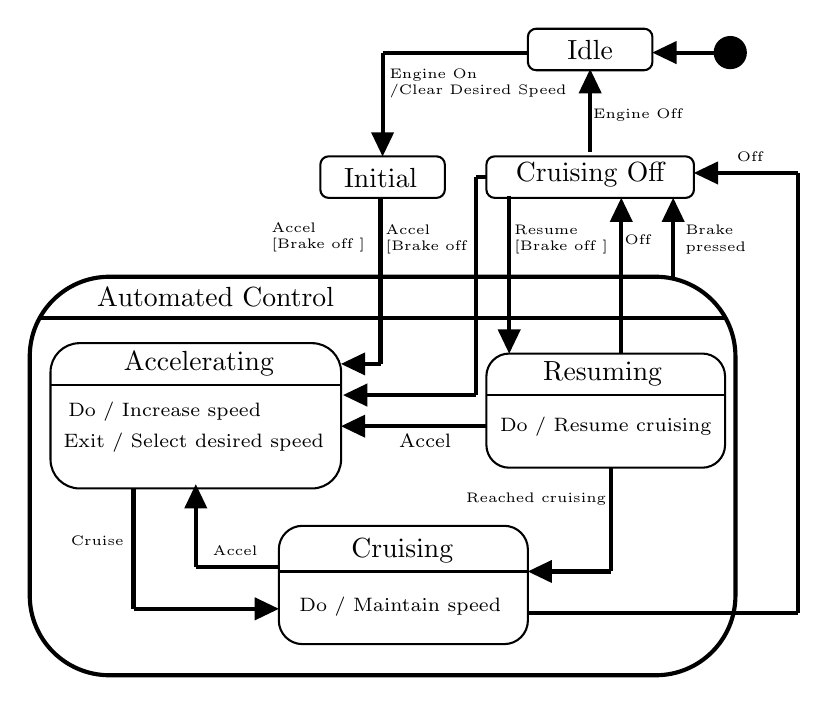
\begin{tikzpicture}[x=0.75pt,y=0.75pt,yscale=-1,xscale=1]
%uncomment if require: \path (0,423); %set diagram left start at 0, and has height of 423

%Rounded Rect [id:dp6662432613291265] 
\draw   (350,77.5) .. controls (350,75.29) and (351.79,73.5) .. (354,73.5) -- (406,73.5) .. controls (408.21,73.5) and (410,75.29) .. (410,77.5) -- (410,89.5) .. controls (410,91.71) and (408.21,93.5) .. (406,93.5) -- (354,93.5) .. controls (351.79,93.5) and (350,91.71) .. (350,89.5) -- cycle ;
%Rounded Rect [id:dp6675663074581135] 
\draw   (330,139) .. controls (330,136.79) and (331.79,135) .. (334,135) -- (426,135) .. controls (428.21,135) and (430,136.79) .. (430,139) -- (430,151) .. controls (430,153.21) and (428.21,155) .. (426,155) -- (334,155) .. controls (331.79,155) and (330,153.21) .. (330,151) -- cycle ;
%Rounded Rect [id:dp4902980476857408] 
\draw   (250,139) .. controls (250,136.79) and (251.79,135) .. (254,135) -- (306,135) .. controls (308.21,135) and (310,136.79) .. (310,139) -- (310,151) .. controls (310,153.21) and (308.21,155) .. (306,155) -- (254,155) .. controls (251.79,155) and (250,153.21) .. (250,151) -- cycle ;
%Rounded Rect [id:dp04982037628337932] 
\draw  [line width=1.5]  (110,231.4) .. controls (110,210.19) and (127.19,193) .. (148.4,193) -- (411.6,193) .. controls (432.81,193) and (450,210.19) .. (450,231.4) -- (450,346.6) .. controls (450,367.81) and (432.81,385) .. (411.6,385) -- (148.4,385) .. controls (127.19,385) and (110,367.81) .. (110,346.6) -- cycle ;
%Straight Lines [id:da7764377667791469] 
\draw [line width=1.5]    (115,213) -- (445,213) ;
%Rounded Rect [id:dp3592571098130719] 
\draw   (120,239) .. controls (120,231.27) and (126.27,225) .. (134,225) -- (246,225) .. controls (253.73,225) and (260,231.27) .. (260,239) -- (260,281) .. controls (260,288.73) and (253.73,295) .. (246,295) -- (134,295) .. controls (126.27,295) and (120,288.73) .. (120,281) -- cycle ;
%Straight Lines [id:da12221010491803885] 
\draw    (120,245) -- (260,245) ;
%Straight Lines [id:da7923623652305394] 
\draw [line width=1.5]    (380,133) -- (380,97) ;
\draw [shift={(380,93)}, rotate = 450] [fill={rgb, 255:red, 0; green, 0; blue, 0 }  ][line width=0.08]  [draw opacity=0] (11.61,-5.58) -- (0,0) -- (11.61,5.58) -- cycle    ;
%Straight Lines [id:da4788139730465273] 
\draw [line width=1.5]    (280,85) -- (280,131) ;
\draw [shift={(280,135)}, rotate = 270] [fill={rgb, 255:red, 0; green, 0; blue, 0 }  ][line width=0.08]  [draw opacity=0] (11.61,-5.58) -- (0,0) -- (11.61,5.58) -- cycle    ;
%Straight Lines [id:da6292308218465252] 
\draw [line width=1.5]    (280,85) -- (350,85) ;
%Straight Lines [id:da0875450823970263] 
\draw [line width=1.5]    (279,155) -- (279,235) ;
%Straight Lines [id:da699195185218056] 
\draw [line width=1.5]    (279,235) -- (264,235) ;
\draw [shift={(260,235)}, rotate = 360] [fill={rgb, 255:red, 0; green, 0; blue, 0 }  ][line width=0.08]  [draw opacity=0] (11.61,-5.58) -- (0,0) -- (11.61,5.58) -- cycle    ;
%Rounded Rect [id:dp8856700522665595] 
\draw   (330,241) .. controls (330,234.92) and (334.92,230) .. (341,230) -- (434,230) .. controls (440.08,230) and (445,234.92) .. (445,241) -- (445,274) .. controls (445,280.08) and (440.08,285) .. (434,285) -- (341,285) .. controls (334.92,285) and (330,280.08) .. (330,274) -- cycle ;
%Straight Lines [id:da9945138562971891] 
\draw    (330,250) -- (445,250) ;
%Straight Lines [id:da6156951818554592] 
\draw [line width=1.5]    (330,265) -- (264,265) ;
\draw [shift={(260,265)}, rotate = 360] [fill={rgb, 255:red, 0; green, 0; blue, 0 }  ][line width=0.08]  [draw opacity=0] (11.61,-5.58) -- (0,0) -- (11.61,5.58) -- cycle    ;
%Rounded Rect [id:dp5701769675760315] 
\draw   (230,324.4) .. controls (230,318.1) and (235.1,313) .. (241.4,313) -- (338.6,313) .. controls (344.9,313) and (350,318.1) .. (350,324.4) -- (350,358.6) .. controls (350,364.9) and (344.9,370) .. (338.6,370) -- (241.4,370) .. controls (235.1,370) and (230,364.9) .. (230,358.6) -- cycle ;
%Straight Lines [id:da16447218181580947] 
\draw    (230,335) -- (350,335) ;
%Straight Lines [id:da8763315052436695] 
\draw [line width=1.5]    (190,333) -- (190,297) ;
\draw [shift={(190,293)}, rotate = 450] [fill={rgb, 255:red, 0; green, 0; blue, 0 }  ][line width=0.08]  [draw opacity=0] (11.61,-5.58) -- (0,0) -- (11.61,5.58) -- cycle    ;
%Straight Lines [id:da04338392142075098] 
\draw [line width=1.5]    (190,333) -- (230,333) ;
%Straight Lines [id:da5695037590069909] 
\draw [line width=1.5]    (160,353) -- (226,353) ;
\draw [shift={(230,353)}, rotate = 180] [fill={rgb, 255:red, 0; green, 0; blue, 0 }  ][line width=0.08]  [draw opacity=0] (11.61,-5.58) -- (0,0) -- (11.61,5.58) -- cycle    ;
%Straight Lines [id:da10244373323079281] 
\draw [line width=1.5]    (160,295) -- (160,353) ;
%Straight Lines [id:da8658544131618406] 
\draw [line width=1.5]    (390,335) -- (354,335) ;
\draw [shift={(350,335)}, rotate = 360] [fill={rgb, 255:red, 0; green, 0; blue, 0 }  ][line width=0.08]  [draw opacity=0] (11.61,-5.58) -- (0,0) -- (11.61,5.58) -- cycle    ;
%Straight Lines [id:da7034657843967269] 
\draw [line width=1.5]    (390,285) -- (390,335) ;
%Straight Lines [id:da5226411692819652] 
\draw [line width=1.5]    (480,143) -- (434,143) ;
\draw [shift={(430,143)}, rotate = 360] [fill={rgb, 255:red, 0; green, 0; blue, 0 }  ][line width=0.08]  [draw opacity=0] (11.61,-5.58) -- (0,0) -- (11.61,5.58) -- cycle    ;
%Straight Lines [id:da01310825459474807] 
\draw [line width=1.5]    (480,143) -- (480,355) ;
%Straight Lines [id:da8077248116651661] 
\draw [line width=1.5]    (350,355) -- (480,355) ;
%Straight Lines [id:da581938331155091] 
\draw [line width=1.5]    (420,193) -- (420,159) ;
\draw [shift={(420,155)}, rotate = 450] [fill={rgb, 255:red, 0; green, 0; blue, 0 }  ][line width=0.08]  [draw opacity=0] (11.61,-5.58) -- (0,0) -- (11.61,5.58) -- cycle    ;
%Straight Lines [id:da5646686872608353] 
\draw [line width=1.5]    (395,230) -- (395,159) ;
\draw [shift={(395,155)}, rotate = 450] [fill={rgb, 255:red, 0; green, 0; blue, 0 }  ][line width=0.08]  [draw opacity=0] (11.61,-5.58) -- (0,0) -- (11.61,5.58) -- cycle    ;
%Straight Lines [id:da777864348657342] 
\draw [line width=1.5]    (341,154) -- (341,226) ;
\draw [shift={(341,230)}, rotate = 270] [fill={rgb, 255:red, 0; green, 0; blue, 0 }  ][line width=0.08]  [draw opacity=0] (11.61,-5.58) -- (0,0) -- (11.61,5.58) -- cycle    ;
%Shape: Circle [id:dp37606004244595703] 
\draw  [fill={rgb, 255:red, 0; green, 0; blue, 0 }  ,fill opacity=1 ] (440,85) .. controls (440,80.86) and (443.36,77.5) .. (447.5,77.5) .. controls (451.64,77.5) and (455,80.86) .. (455,85) .. controls (455,89.14) and (451.64,92.5) .. (447.5,92.5) .. controls (443.36,92.5) and (440,89.14) .. (440,85) -- cycle ;
%Straight Lines [id:da3457264380323728] 
\draw [line width=1.5]    (440,85) -- (414,85) ;
\draw [shift={(410,85)}, rotate = 360] [fill={rgb, 255:red, 0; green, 0; blue, 0 }  ][line width=0.08]  [draw opacity=0] (11.61,-5.58) -- (0,0) -- (11.61,5.58) -- cycle    ;
%Straight Lines [id:da19616464722638915] 
\draw [line width=1.5]    (325,250) -- (265,250) ;
\draw [shift={(261,250)}, rotate = 360] [fill={rgb, 255:red, 0; green, 0; blue, 0 }  ][line width=0.08]  [draw opacity=0] (11.61,-5.58) -- (0,0) -- (11.61,5.58) -- cycle    ;
%Straight Lines [id:da6702411290187669] 
\draw [line width=1.5]    (325,145) -- (325,250) ;
%Straight Lines [id:da7965543187487978] 
\draw [line width=1.5]    (325,145) -- (330,145) ;

% Text Node
\draw (380,83.5) node   [align=left] {Idle};
% Text Node
\draw (380,143.74) node   [align=left] {Cruising Off};
% Text Node
\draw (279,145.5) node   [align=left] {Initial};
% Text Node
\draw (199.5,202.5) node   [align=left] {Automated Control};
% Text Node
\draw (191.5,235) node   [align=left] {Accelerating};
% Text Node
\draw (386,239.5) node   [align=left] {Resuming};
% Text Node
\draw (289.5,325) node   [align=left] {Cruising};
% Text Node
\draw (326,100) node  [font=\tiny] [align=left] {Engine On\\/Clear Desired Speed};
% Text Node
\draw (142.5,320) node  [font=\tiny] [align=left] {Cruise};
% Text Node
\draw (209,325) node  [font=\tiny] [align=left] {Accel};
% Text Node
\draw (300.5,272) node  [font=\scriptsize] [align=left] {Accel};
% Text Node
\draw (457,135) node  [font=\tiny] [align=left] {Off};
% Text Node
\draw (366,175) node  [font=\tiny] [align=left] {Resume\\\lbrack Brake off \rbrack };
% Text Node
\draw (440.5,175) node  [font=\tiny] [align=left] {Brake\\pressed};
% Text Node
\draw (175,258) node  [font=\scriptsize] [align=left] {Do / Increase speed};
% Text Node
\draw (189,273) node  [font=\scriptsize] [align=left] {Exit / Select desired speed};
% Text Node
\draw (288.5,352) node  [font=\scriptsize] [align=left] {Do / Maintain speed};
% Text Node
\draw (387.5,265) node  [font=\scriptsize] [align=left] {Do / Resume cruising};
% Text Node
\draw (403,115) node  [font=\tiny] [align=left] {Engine Off};
% Text Node
\draw (354,300) node  [font=\tiny] [align=left] {Reached cruising};
% Text Node
\draw (249,174) node  [font=\tiny] [align=left] {Accel\\\lbrack Brake off \rbrack };
% Text Node
\draw (304,175) node  [font=\tiny] [align=left] {Accel\\\lbrack Brake off \rbrack };
% Text Node
\draw (403,175) node  [font=\tiny] [align=left] {Off};


\end{tikzpicture}
    \caption{Cruise control FSM example}
    \label{fig:fsmej}
\end{figure}

The behavior of this system is state-dependent in that the executed actions correspond not only to the driver input, but also on the current state of the system and with the status of the engine and the brake. 
The figure \ref{fig:fsmej} illustrate the modeling of this system with the "Automated Control" state acting as composite.
\medskip

\begin{tcolorbox}
\HandRight Transitions to a specific state inside a composite state and vice versa, should be parametrized in the last two parameters of the transition entry. Please see the transition layout in table \ref{ttable_layout}.
\end{tcolorbox}



Before getting started, the required user-defined signals, variables, and transition tables should be defined:

\lstinputlisting[style=CStyle]{sec3fsmcruisectrlttabledef.c}

Then, signal-actions and state callbacks are later defined:

\lstinputlisting[style=CStyle]{sec3fsmcruisectrlstates.c}

Finally, the dedicated task for the FSM and related objects are configured.

\lstinputlisting[style=CStyle]{sec3fsmcruisectrlsetup.c}

\subsection{Co-Routines}
As showed in figure \ref{fig:coroutine}, a task coded as a Co-Routine, is just a task that allows multiple entry points for suspending and resuming execution at certain locations, this feature can bring benefits by improving the task cooperative scheme and providing a linear code execution for event-driven systems without complex state machines or full multi-threading.
\medskip

\begin{figure}[H]
    \centering
    \begin{tikzpicture}[x=0.75pt,y=0.75pt,yscale=-1,xscale=1,scale=1]
        \foreach \x in {100,120,160,180,220}{ \draw    (121,\x) -- (191,\x) ; }
        \foreach \x in {100,120,140,180,200,220}{ \draw    (331,\x) -- (401,\x) ; }
        \draw   (290,70) -- (430,70) -- (430,250) -- (290,250) -- cycle ;
        \draw   (80,70) -- (220,70) -- (220,250) -- (80,250) -- cycle ;
        
        \draw  [fill=lightgray  ,fill opacity=1 ] (290,46) .. controls (290,42.69) and (292.69,40) .. (296,40) -- (424,40) .. controls (427.31,40) and (430,42.69) .. (430,46) -- (430,70) .. controls (430,70) and (430,70) .. (430,70) -- (290,70) .. controls (290,70) and (290,70) .. (290,70) -- cycle ;
        \draw  [fill=lightgray  ,fill opacity=1 ] (80,46) .. controls (80,42.69) and (82.69,40) .. (86,40) -- (214,40) .. controls (217.31,40) and (220,42.69) .. (220,46) -- (220,70) .. controls (220,70) and (220,70) .. (220,70) -- (80,70) .. controls (80,70) and (80,70) .. (80,70) -- cycle ;
        \draw    (210,90) -- (210,130) -- (310,90) -- (310,150) -- (210,140) -- (210,200) -- (310,160) -- (310,230) -- (210,210) -- (210,238) ;
        \draw [shift={(210,240)}, rotate = 270] [fill=black  ][line width=0.75]  [draw opacity=0] (8.93,-4.29) -- (0,0) -- (8.93,4.29) -- cycle    ;
        \draw [shift={(210,90)}, rotate = 90] [color=black  ][fill=black  ][line width=0.75]      (0, 0) circle [x radius= 3.35, y radius= 3.35]   ;
        \draw (145,55) node  [align=left] {Task A};
        \draw (127,86) node [scale=0.7, font=\ttfamily] [align=left] {\ttfamily{qCR_Begin\{}};
        \draw (127,234) node [scale=0.7] [align=left] {\ttfamily{\}qCR_End;}};
        \draw (141.5,136) node [scale=0.7] [align=left] {\ttfamily{qCR_Yield;}};
        \draw (141.5,204) node [scale=0.7] [align=left] {\ttfamily{qCR_Yield;}};
        \draw (355,55) node  [align=left] {Task B};
        \draw (337,86) node [scale=0.7] [align=left] {\ttfamily{qCR_Begin\{}};
        \draw (337,234) node [scale=0.7] [align=left] {\ttfamily{\}qCR_End;}};
        \draw (350.5,156) node [scale=0.7] [align=left] {\ttfamily{qCR_Yield;}};
    \end{tikzpicture}
    \caption{Coroutines in QuarkTS}
    \label{fig:coroutine}
\end{figure}
    
The QuarkTS implementation uses the Duff's device approach, and is heavily inspired by the Knuth approach\cite{knuth}, Simon Tatham's Co-Routines in C \cite{tatham} and Adam Dunkels Protothreads \cite{dunkels}. This means that a \textit{local-continuation} variable is used to preserve the current state of execution at a particular place of the Co-Routine scope but without any call history or local variables. This brings benefits to lower RAM usage, but at the cost of some restrictions on how a Co-routine can be used.
\medskip

\textbf{Limitations and Restrictions}:

\begin{itemize}
    \item The stack of a Co-Routine  is not maintained when a yield is performed. This means variables allocated on the stack will loose their values. To overcome this, a variable that must maintain its value across a blocking call must be declared as \lstinline{static}.
    \item Calls to API functions that could cause the Co-Routine to block, can only be made from the Co-Routine  function itself - not from within a function called by the Co-Routine .
    \item The implementation does not permit yielding or blocking calls to be made from within a \lstinline{switch} statement.
\end{itemize}

\subsubsection{Coding a Co-Routine}
The application writer just needs to create the body of the Co-Routine . This means starting a Co-Routine segment with \lstinline{qCR_Begin} \index{\lstinline{qCR_Begin}} and end with \lstinline{qCR_End} statement \index{\lstinline{qCR_End}}. From now on, yields and blocking calls from the Co-Routine scope are allowed.
\medskip

\lstinputlisting[style=CStyle]{sec3coroutinecoding.c}  

The \lstinline{qCR_Begin} statement should be placed at the start of the task function in which the Co-routine runs. All C statements above the \lstinline{qCR_Begin} will be executed as if they were in an endless-loop each time the task is scheduled.

A \lstinline{qCR_Yield} \index{\lstinline{qCR_Yield}} statement return the CPU control back to the scheduler but saving the execution progress, thereby allowing other processing tasks to take place in the system. With the next task activation, the Co-Routine will resume the execution after the last \lstinline{qCR_Yield} statement.
\medskip

\begin{tcolorbox}
\HandRight All the Co-routine statements has the \textit{qCR} appended at the beginning of their name.
\end{tcolorbox}

\begin{tcolorbox}
\HandRight Co-Routine statements can only be invoked from the scope of the Co-Routine.
\end{tcolorbox}


\begin{tcolorbox}
\HandRight Do not use an endless-loop inside a Co-routine ,this behavior it's already hardcoded within the segment definition.
\end{tcolorbox}

\subsubsection{Blocking calls}
Blocking calls inside a Co-Routine should be made with the provided statements, all of them with a common feature: an implicit yield.

A widely used procedure is to wait for a fixed period of time. For this, the \lstinline{qCR_Delay()} should be used \index{\lstinline{qCR_Delay}}. 
\medskip


\begin{lstlisting}[style=CStyle]
qCR_Delay( qTime_t tDelay ) 
\end{lstlisting}

As expected, this statement makes an apparent blocking over the application flow, but to be precise, a yield is performed until the requested time expires, this allows other tasks to be executed until the blocking call finish. This \textit{"yielding until condition meet"} behavior its the common pattern among the other blocking statements.
\medskip

Another common blocking call is \lstinline{qCR_WaitUntil()} \index{\lstinline{qCR_WaitUntil}}:

\begin{lstlisting}[style=CStyle]
qCR_WaitUntil( Condition ) 
\end{lstlisting}

This statement takes a \lstinline{Condition} argument, a logical expression that will be performed when the Co-Routine resumes their execution. As mentioned before, this type of statement exposes the expected behavior, yielding until the condition is met.
\medskip

An additional wait statement is also provided that sets a timeout for the logical condition to be met, with a similar behavior of \lstinline{qCR_WaitUntil}. \index{\lstinline{qCR_TimedWaitUntil}}
\medskip

\begin{lstlisting}[style=CStyle]
qCR_TimedWaitUntil( Condition, qTime_t Timeout )
\end{lstlisting}

Optionally, the \lstinline{Do-Until} \index{\lstinline{qCR_Do}} \index{\lstinline{qCR_Until}} structure gives to application writer the ability to perform a multi-line job before the yield, allowing more complex actions to being performed after the Co-Routine resumes: 
\medskip

\begin{lstlisting}[style=CStyle]
qCR_Do{
    /* Job : a set of instructions*/
}qCR_Until( Condition );
\end{lstlisting}

\subsubsection*{Usage example:}
\lstinputlisting[style=CStyle]{sec3coroutinedem1.c}

\subsubsection{Positional jumps}
This feature provides positional local jumps, control flow that deviates from the usual Co-Routine call. 

The complementary statements \lstinline{qCR_PositionGet()} \index{\lstinline{qCR_PositionGet}} and \lstinline{qCR_PositionRestore()} \index{\lstinline{qCR_PositionRestore}} provide this functionality.
The first one saves the Co-Routine state at some point of their execution into \lstinline{CRPos}, a variable of type \lstinline{qCR_Position_t} \index{\lstinline{qCR_Position_t}},  that can be used at some later point of program execution by \lstinline{qCR_PositionRestore()} to restore the Co-Routine  state to the one saved by \lstinline{qCR_PositionGet()} into \lstinline{CRPos}. This process can be imagined to be a "jump" back to the point of program execution where \lstinline{qCR_PositionGet()} saved the Co-Routine  environment.
\medskip

\begin{lstlisting}[style=CStyle]
qCR_PositionGet( qCR_Position_t CRPos )
\end{lstlisting}

\begin{lstlisting}[style=CStyle]
qCR_PositionRestore( qCR_Position_t CRPos )
\end{lstlisting}

And to reset the \lstinline{CRPos} variable to the beginning of the Co-Routine, use \index{\lstinline{qCR_PositionReset}}:

\begin{lstlisting}[style=CStyle]
qCR_PositionReset( qCR_Position_t CRPos )
\end{lstlisting}

\subsubsection{Semaphores}
This module implements counting semaphores on top of Co-Routines. Semaphores are a synchronization primitive that provide two operations: \textit{wait} and \textit{signal}. The \textit{wait} operation checks the semaphore counter and blocks the Co-Routine if the counter is zero. The \textit{signal} operation increases the semaphore counter but does not block. If another Co-Routine has blocked waiting for the semaphore that is signaled, the blocked Co-Routines will become runnable again.

Semaphores are referenced by handles, a variable of type \lstinline{qCR_Semaphore_t} \index{\lstinline{qCR_Semaphore_t}}and must be initialized with \lstinline{qCR_SemInit()} \index{\lstinline{qCR_SemInit}} before any usage.  Here, a value for the counter is required. Internally, semaphores use an \lstinline{unsigned int} to represent the counter, therefore the \lstinline{Value} argument should be within range of this data-type.
\medskip

\begin{lstlisting}[style=CStyle]
qCR_SemInit( qCR_Semaphore_t *sem, qUINT16_t Value )
\end{lstlisting}

To perform the \textit{wait} operation, the \lstinline{qCR_SemWait()} \index{\lstinline{qCR_SemWait}} statement should be used. The wait operation causes the Co-routine to block while the counter is zero. When the counter reaches a value larger than zero, the Co-Routine will continue.
\medskip


\begin{lstlisting}[style=CStyle]
qCR_SemWait( qCR_Semaphore_t *sem )
\end{lstlisting}

Finally, \lstinline{qCR_SemSignal()} \index{\lstinline{qCR_SemSignal}} carries out the \textit{signal} operation on the semaphore. This signaling increments the counter inside the semaphore, which eventually will cause waiting Co-routines to continue executing.
\medskip

\begin{lstlisting}[style=CStyle]
qCR_SemSignal( qCR_Semaphore_t *sem )
\end{lstlisting}


\subsubsection*{Usage example:}
The following example shows how to implement the bounded buffer problem using Co-Routines and semaphores. The example uses two tasks: one that produces items and other that consumes items.

Note that there is no need for a mutex to guard the \lstinline{add_to_buffer()} and \lstinline{get_from_buffer()} functions because of the implicit locking semantics of Co-Routines, so it will never be preempted and will never block except in an explicit \lstinline{qCR_SemWait} statement.
\medskip

\lstinputlisting[style=CStyle]{sec3coroutinedem2.c}

\subsubsection{External control}
There are several circumstances where becomes necessary to control the flow of execution outside the segment that defines the Co-routine itself. This is usually used to defer the job of the Co-routine or resume it in response to specific occurrences that arises in other contexts, either tasks or interrupts.

To code this specific situations, a handler to the Co-routine should be defined, a variable of type \lstinline{qCR_Handle_t}. In addition to this, the scope of the target Co-routine must be started with the \lstinline{qCR_BeginWithHandle} statement instead of \lstinline{qCR_Begin}.
\medskip

\lstinputlisting[style=CStyle]{sec3coroutinectrlext.c}

As seen in the code snippet above, the Co-routine handle its globally declared to allow other contexts to access it.  The example shows that another task can control the Co-routine using the \lstinline{qCR_ExternControl} API. The actions performed by this API can be only be effective after the handle instantiation, an operation that takes place once on the first call of the Co-routine.
\medskip

\begin{lstlisting}[style=CStyle]
void qCR_ExternControl( qCR_Handle_t h, const qCR_ExternAction_t action,  
                        const qCR_ExtPosition_t action )                      
\end{lstlisting}\index{\lstinline{qCR_ExternControl}}

\subsubsection*{Parameters}
\begin{itemize}
    \item \lstinline{h} : The Co-routine handle.
    \item \lstinline{action} : The specific action to perform, should be one of the following:
    \begin{itemize}
        \item \lstinline{qCR_RESTART} : Restart the Co-routine execution at the place of the \lstinline{qCR_BeginWithHandle} statement.  
        \item \lstinline{qCR_SUSPEND} :  Suspend the entire Co-routine segment. The task will still running instructions outside the segment.
        \item \lstinline{qCR_RESUME} : Resume the entire Co-routine segment at the point where it had been left before the suspension.
        \item \lstinline{qCR_POSITIONSET} : Force the coroutine execution at the position specified in \lstinline{pos}. If a non-valid position is supplied, the Co-routine segment will be suspended.      
    \end{itemize}
    \item \lstinline{pos} : The requested position if action = \lstinline{qCR_POSITIONSET}. For other actions this argument its ignored.  
\end{itemize}

\hrulefill
\medskip

\begin{tcolorbox}
\HandRight A \lstinline{NULL} initialization its mandatory on \lstinline{qCR_Handle_t} variables. Undefined behavior may occur if this step is ignored.
\end{tcolorbox}

\subsection{AT Command Line Interface} 
A command-line interface (CLI) is a way to interact directly with the software of an embedded system in the form of text commands and responses. It can be seen as a typed set of commands to produce a result, but here, the commands are typed in real-time by a user through a specific interface, for example, UART, USB, LAN, etc. 

A CLI is often developed to aid initial driver development and debugging. This CLI might become the interface (or one of the interfaces) used by a sophisticated end-user to interact with the product. Think of typing commands to control a machine, or perhaps for low-level access to the control system as a development tool, tweaking time-constants and monitoring low-level system performance during testing. 

\subsubsection{The components of the CLI}
The provided development API parses and handles input commands, following a simplified form of the extended AT-commands syntax. 

\begin{figure}[H]
    \centering
    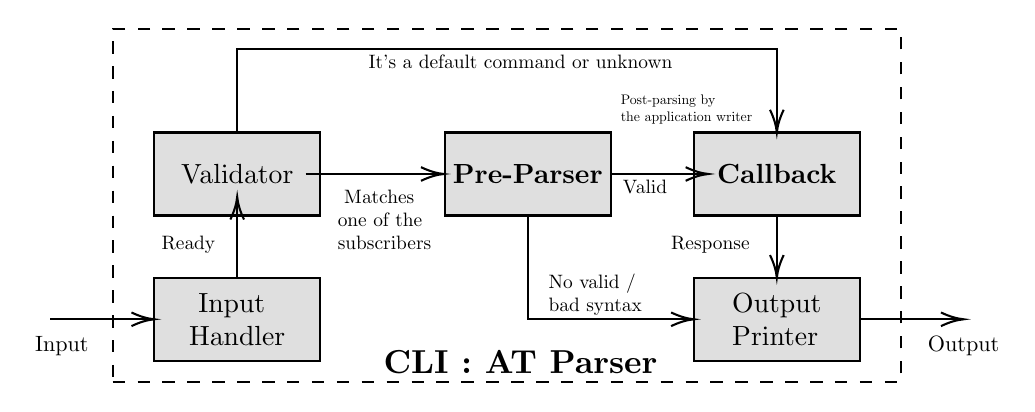
\begin{tikzpicture}[x=0.75pt,y=0.75pt,scale=1]
        \draw  [color=black  ,draw opacity=1 ][fill=white  ,fill opacity=1 ][dash pattern={on 4.5pt off 4.5pt}] (80,70) -- (460,70) -- (460,240) -- (80,240) -- cycle ;
        \draw  [fill=lightgray!50  ,fill opacity=1 ] (100,80) -- (180,80) -- (180,120) -- (100,120) -- cycle ;
        \draw  [fill=lightgray!50  ,fill opacity=1 ] (100,150) -- (180,150) -- (180,190) -- (100,190) -- cycle ;
        \draw  [fill=lightgray!50  ,fill opacity=1 ] (240,150) -- (320,150) -- (320,190) -- (240,190) -- cycle ;
        \draw  [fill=lightgray!50  ,fill opacity=1 ] (360,150) -- (440,150) -- (440,190) -- (360,190) -- cycle ;
        \draw  [fill=lightgray!50  ,fill opacity=1 ] (360,80) -- (440,80) -- (440,120) -- (360,120) -- cycle ;
        \draw    (140,190) -- (140,230) -- (400,230) -- (400,192) ;
        \draw [shift={(400,190)}, rotate = 450] [color=black ][line width=0.75]    (10.93,-3.29) .. controls (6.95,-1.4) and (3.31,-0.3) .. (0,0) .. controls (3.31,0.3) and (6.95,1.4) .. (10.93,3.29)   ;
        \draw    (50,100) -- (98,100) ;
        \draw [shift={(100,100)}, rotate = 180] [color=black ][line width=0.75]    (10.93,-3.29) .. controls (6.95,-1.4) and (3.31,-0.3) .. (0,0) .. controls (3.31,0.3) and (6.95,1.4) .. (10.93,3.29)   ;
        \draw    (440,100) -- (488,100) ;
        \draw [shift={(490,100)}, rotate = 180] [color=black ][line width=0.75]    (10.93,-3.29) .. controls (6.95,-1.4) and (3.31,-0.3) .. (0,0) .. controls (3.31,0.3) and (6.95,1.4) .. (10.93,3.29)   ;
        \draw    (400,150) -- (400,122) ;
        \draw [shift={(400,120)}, rotate = 450] [color=black ][line width=0.75]    (10.93,-3.29) .. controls (6.95,-1.4) and (3.31,-0.3) .. (0,0) .. controls (3.31,0.3) and (6.95,1.4) .. (10.93,3.29)   ;
        \draw    (280,150) -- (280,100) -- (358,100) ;
        \draw [shift={(360,100)}, rotate = 180] [color=black ][line width=0.75]    (10.93,-3.29) .. controls (6.95,-1.4) and (3.31,-0.3) .. (0,0) .. controls (3.31,0.3) and (6.95,1.4) .. (10.93,3.29)   ;
        \draw (400,170) node  [align=left] {\textbf{Callback}};
        \draw (280,170) node  [align=left] {\textbf{Pre-Parser}};
        \draw (140,170) node  [align=left] {Validator};
        \draw (400,100) node  [align=left] {Output\\Printer};
        \draw (140,100) node  [align=left] { \ Input\\Handler};
        \draw (55.5,87) node [scale=0.8] [align=left] {Input};
        \draw (490,87) node [scale=0.8] [align=left] {Output};
        \draw (368,136) node [scale=0.7] [align=left] {Response};
        \draw (336.5,164) node [scale=0.7] [align=left] {Valid};
        \draw (211,148) node [scale=0.7] [align=left] { \ Matches\\ one of the\\subscribers};
        \draw (276.5,224) node [scale=0.7] [align=left] {It's a default command or unknown};
        \draw (312.5,112) node [scale=0.7] [align=left] {No valid /\\bad syntax};
        \draw (356.5,201) node [scale=0.5] [align=left] {Post-parsing by \\the application writer};
        \draw (116.5,136) node [scale=0.7] [align=left] {Ready};
        \draw (276.5,79.5) node [scale=1.2] [align=left] {\textbf{CLI : AT Parser}};
        \draw    (173,170) -- (237.5,170) ;
        \draw [shift={(239.5,170)}, rotate = 180] [color=black ][line width=0.75]    (10.93,-3.29) .. controls (6.95,-1.4) and (3.31,-0.3) .. (0,0) .. controls (3.31,0.3) and (6.95,1.4) .. (10.93,3.29)   ;
        \draw    (320.5,170) -- (365,170) ;
        \draw [shift={(367,170)}, rotate = 180] [color=black ][line width=0.75]    (10.93,-3.29) .. controls (6.95,-1.4) and (3.31,-0.3) .. (0,0) .. controls (3.31,0.3) and (6.95,1.4) .. (10.93,3.29)   ;
        \draw    (140,120) -- (140,157) ;
        \draw [shift={(140,159)}, rotate = 270] [color=black ][line width=0.75]    (10.93,-3.29) .. controls (6.95,-1.4) and (3.31,-0.3) .. (0,0) .. controls (3.31,0.3) and (6.95,1.4) .. (10.93,3.29)   ;
    \end{tikzpicture}
    \caption{AT parser for a CLI implementation}
    \label{fig:atparser}
\end{figure}

As seen in figure \ref{fig:atparser}, the CLI has a few components described below:
\begin{itemize}
    \item  \textit{Input Handler} : It is responsible for collecting incoming data from the \textit{input} in the form of ASCII characters inside a buffer. When this buffer is ready by receiving an \lstinline{EOL}(\textit{End-Of-Line}) byte, it notifies the \textit{validator} to perform the initial checks.
    \item \textit{Validator}: Take the input string and perform three checks over it:
    \begin{enumerate}
        \item The input matches one of the subscribed commands.
        \item The input matches one of the default commands.
        \item The input is unknown
    \end{enumerate}
    \item \textit{Pre-Parser}: Takes the input if the \textit{validator} asserts the first check. It is responsible for syntax validation and classification. Also, prepares the input argument for the next component.
    \item \textit{Callback or Post-Parser}: If input at the \textit{pre-parser} is valid, the respective command-callback is invoked. Here, the application writer is free to handle the command execution and the output response.
    \item \textit{Output printer} : Takes all the return status of the previous components to print out a response at the output.
\end{itemize}
\bigskip

\begin{tcolorbox}
\HandRight Here, \textit{Input} and \textit{Output} should be provided by the application writer, for example, if a UART interface is chosen, the input should take the received bytes from an ISR and the output is a function to print out a single byte.
\end{tcolorbox}

\subsubsection{Supported syntax} \label{atsyntax}

The syntax is straightforward and the rules are provided below:

\begin{itemize}
    \item All command lines must start with \lstinline{AT} and end with an \lstinline{EOL} character. By default, the CLI uses the carriage return character. (We will use \lstinline{<CR>} to represent a carriage return character in this document).
    \item AT commands are case-insensitive 
    \item Only four types of AT commands are allowed:
    \begin{itemize}
        \item \textbf{Acting} (\lstinline{QATCLI_CMDTYPE_ACT}) : This is the simplest type of commands that can be subscribed. Its normally used to execute the action that the command should do. This type doesn't take arguments or modifiers, for example,
        \begin{lstlisting}
        AT+CMD
        \end{lstlisting}
        \item \textbf{Read} (\lstinline{QATCLI_CMDTYPE_READ}) : This type of command allows you to read or test a value already configured for the specified parameter. Only one argument is allowed.
        \begin{lstlisting}
        AT+CMD?
        AT+CMD?PARAM1
        \end{lstlisting}        
        \item \textbf{Test} (\lstinline{QATCLI_CMDTYPE_TEST}) : These types of commands allow you to get the values that can be set for its parameters. No parameters are allowed here.
        \begin{lstlisting}
        AT+CMD=?
        \end{lstlisting}
        \item \textbf{Parameter Set} (\lstinline{QATCLI_CMDTYPE_PARA}) : These types of commands allow \textit{n} arguments to be passed for setting parameters, for example:
        \begin{lstlisting}
        AT+CMD=x,y
        \end{lstlisting}
    \end{itemize}
    If none of the types is given at the input, the command response will be \lstinline{ERROR}
    \item The possible output responses are:
    \begin{itemize}
        \item \lstinline{OK}: Indicates the successful execution of the command.
        \item \lstinline{ERROR}: A generalized message to indicate failure in executing the command. 
        \item \lstinline{UNKNOWN} : The input command its not subscribed.
        \item \lstinline{NOT ALLOWED} : The command syntax is not one of the allowed types.
        \item \lstinline{User-defined}: A custom output message defined by the application writer.
        \item \lstinline{NONE} : No response.
    \end{itemize}
\end{itemize}

All responses are followed by a \lstinline{<CR><LF>}.
\medskip

Errors generated during the execution of these AT commands could be due to the following reasons:
\begin{itemize}
    \item Incorrect syntax/parameters of the AT command
    \item Bad parameters or not allowed operations defined by the application writer.
\end{itemize}

In case of an error, the string \lstinline{ERROR} or \lstinline{ERROR:<error_no>} are displayed.

\subsubsection{Setting up an AT-CLI instance}
Before starting the CLI development, the corresponding instance must be defined; a data structure of type \lstinline{qATCLI_t} \index{\lstinline{qATCLI_t}}. 
The instance should be initialized using the \lstinline{qATCLI_Setup()} API \index{\lstinline{qATCLI_Setup}}. A detailed description of this function is shown bellow:
\medskip

\begin{lstlisting}[style=CStyle]
qBool_t qATCLI_Setup( qATCLI_t * const cli, const qPutChar_t OutputFcn, 
                      char *Input, const size_t SizeInput, char *Output, 
                      const size_t SizeOutput, const char *Identifier, 
                      const char *OK_Response, const char *ERROR_Response, 
                      const char *NOTFOUND_Response, const char *term_EOL )
\end{lstlisting}

\subsubsection*{Parameters}
\begin{itemize}
    \item \lstinline{cli} : A pointer to the AT Command Line Interface instance. 
    \item \lstinline{OutputFcn} : The basic output-char wrapper function. All the CLI responses  will be printed-out through this function.
    \item \lstinline{Input} : A memory location to store the parser input (mandatory) 
    \item \lstinline{SizeInput} : The size of the memory allocated in \lstinline{Input}. 
    \item \lstinline{Output} : A memory location to store the parser output. If not used, pass \lstinline{NULL}.
    \item \lstinline{SizeOutput} : The size of the memory allocated in \lstinline{Output}. 
    \item \lstinline{Identifier} : The device identifier string. This string will be printed-out after a call to the \lstinline{AT_DEFAULT_ID_COMMAND}.
    \item \lstinline{OK_Response} : The output message when a command callback returns \lstinline{QATCLI_OK}. To use the default, pass \lstinline{NULL}.
    \item \lstinline{ERROR_Response} : The output message when a command callback returns \lstinline{QATCLI_ERROR} or any \lstinline{QATCLI_ERRORCODE(#)}. To use the default, pass \lstinline{NULL}.
    \item \lstinline{NOTFOUND_Response } : The output message when input doesn't match with any of  the available commands. To use the default, pass \lstinline{NULL}.
    \item \lstinline{term_EOL} : The \textit{End-Of-Line} string printed out after any of the parser messages. To use the default, pass \lstinline{NULL}. 
\end{itemize}

\subsubsection{Subscribing commands to the parser}
The AT CLI is able to subscribe any number of custom AT commands. For this, the 
\lstinline{qATCLI_CmdSubscribe()} \index{\lstinline{qATCLI_CmdSubscribe}} API should be used.

This function subscribes the CLI instance to a specific command with an associated callback function, so that next time the required command is sent to the CLI input, the callback function will be executed.
\medskip
The CLI module only analyzes commands that follow the simplified AT-Commands syntax already described in section \ref{atsyntax}.
\medskip

\begin{lstlisting}[style=CStyle]
qBool_t qATCLI_CmdSubscribe( qATCLI_t * const cli, 
                             qATCLI_Command_t * const Command, 
                             const char *TextCommand, 
                             qATCLI_CommandCallback_t Callback, 
                             qATCLI_Options_t CmdOpt, void *param )
\end{lstlisting}

\subsubsection*{Parameters}
\begin{itemize}
    \item \lstinline{cli} : A pointer to the AT Command Line Inteface instance. 
    \item \lstinline{Command} :  A pointer to the AT command object.
    \item \lstinline{TextCommand} : The string (name) of the command we want to subscribe to. Since this service only handles AT commands, this string has to begin by the \lstinline{"at"} characters and should be in lower case.
    \item \lstinline{Callback} : The handler of the callback function associated to the command. Prototype: 
    \lstinline{qATCLI_Response_t xCallback(qATCLI_Handler_t, qATCLI_PreCmd_t )}
    \item \lstinline{CmdOpt} : This flag combines with a bitwise ‘OR’ (‘|’) the following information:
    \begin{itemize}
        \item \lstinline{QATCLI_CMDTYPE_PARA} : \lstinline{AT+cmd=x,y} is allowed. The execution of the callback function also depends on whether the number of argument is valid or not. Information about number of arguments is combined with a bitwise 'OR' : \lstinline{QATCLI_CMDTYPE_PARA | 0xXY} , where \lstinline{X} which defines maximum argument number for incoming command and \lstinline{Y} which defines minimum argument number for incoming command.
        \item \lstinline{QATCLI_CMDTYPE_TEST} : \lstinline{AT+cmd=?} is allowed. 
        \item \lstinline{QATCLI_CMDTYPE_READ} : \lstinline{AT+cmd?} is allowed. 
        \item \lstinline{QATCLI_CMDTYPE_ACT} : \lstinline{AT+cmd} is allowed. 
    \end{itemize}
    \item \lstinline{param} :  User storage pointer.
\end{itemize}

\subsubsection{Writing a command callback}
The command callback should be coded by the application writter. Here, the following prototype should be used:
\medskip

\begin{lstlisting}[style=CStyle]
qATCLI_Response_t CMD_Callback( qATCLI_Handler_t h ){
    /* TODO : The command callback */
}
\end{lstlisting}

The callback takes one argument of type \lstinline{qATCLI_Handler_t} and returns a single value.
\medskip
The input argument it's just a pointer to public data of the CLI instance where the command it subscribed to. From the callback context, can be used to print out extra information as a command response, parse the command parameters, and query properties with crucial information about the detected command, like the type, the number of arguments, and the subsequent string after the command text. The members are described as follows:

\begin{itemize}
    \item \lstinline{Command} (read-only) : A pointer to the calling AT Command object.
    \item \lstinline{Type} (read-only) : The command type.
    \item \lstinline{StrData} (read-only) : The string data after the command text.
    \item \lstinline{StrLen} (read-only) : The length of \lstinline{StrData}.
    \item \lstinline{NumArgs} (read-only) : Number of arguments, only available if \lstinline{Type = QATCLI_CMDTYPE_PARA}.
    \item \lstinline{Output} : Points to the output buffer storage area.
    \item \lstinline{UserData} : Points to the user-defined data - Storage Pointer
    
    This argument also includes helper methods to write the output and retrieve command arguments:
    
    \item \lstinline{void puts(const char* s)} : Writes the string \lstinline{s} to the output.
    \item \lstinline{void putch(const char c)} : Writes the byte \lstinline{c} to the output.
    \item \lstinline{char* GetArgPtr( qIndex_t n )} : Get the pointer where the desired argument starts.
    \item \lstinline{int GetArgInt( qIndex_t n )} : Get the \lstinline{n} argument parsed as integer.
    \item \lstinline{qUINT32_t GetArgHex( qIndex_t n )} : Get the \lstinline{n} HEX argument parsed as \lstinline{qUINT32_t}.
    \item \lstinline{qFloat32_t GetArgFlt( qIndex_t n )} : Get the \lstinline{n} argument parsed as float.
    \item \lstinline{char* GetArgString( qIndex_t n, char *out )} :  get the argument \lstinline{n} by copying the string into \lstinline{out}.
\end{itemize}

The return value (an enum of type \lstinline{qATCLI_Response_t}) \index{\lstinline{qATCLI_Response_t}} determines the response shown by the \textit{Output printer} component. The possible allowed values are:

\begin{itemize}
    \item \lstinline{QATCLI_OK} : as expected, print out the \lstinline{OK} string.
    \item \lstinline{QATCLI_ERROR} : as expected, print out the \lstinline{ERROR} string.
    \item \lstinline{QATCLI_ERRORCODE(no)} : Used to indicate an error code. This code is defined by the application writer and should be a value between 1 and 32766. For example, a return value of \lstinline{QATCLI_ERRORCODE(15)}, will print out the string \lstinline{ERROR:15}.
    \item \lstinline{QATCLI_NORESPONSE} : No response will be printed out.
\end{itemize}


A simple example of how the command callback should be coded is showed below:
\medskip

\lstinputlisting[style=CStyle]{sec3atclicallback.c}


\subsubsection{Handling the input}
Input handling is simplified using the provided APIs. The \lstinline{qATCLI_ISRHandler()} \index{\lstinline{qATCLI_ISRHandler}} and \lstinline{qATCLI_ISRHandlerBlock()}  \index{\lstinline{qATCLI_ISRHandlerBlock}} functions are intended to be used from the interrupt context. This avoids any kind of polling implementation and allows the CLI application to be designed using an event-driven pattern.
\medskip
\begin{lstlisting}[style=CStyle]
qBool_t qATCLI_ISRHandler( qATCLI_t * const cli, char c )
\end{lstlisting}

\begin{lstlisting}[style=CStyle]
qBool_t qATCLI_ISRHandlerBlock( qATCLI_t * const cli, char *data, 
                                const size_t n )
\end{lstlisting}

Both functions feed the parser input, the first one with a single character and the second with a string. The application writer should call one of these functions from the desired hardware interface, for example, from a UART receive ISR. 

\subsubsection*{Parameters}
\begin{itemize}
    \item \lstinline{cli} : Both APIs take a pointer to AT Command Line Interface instance.
\end{itemize}

for \lstinline{qATCLI_ISRHandler} :
\begin{itemize}
    \item \lstinline{c} : The incoming byte/char to the input. 
\end{itemize}

for \lstinline{qATCLI_ISRHandlerBlock} :
\begin{itemize}
    \item \lstinline{data} : The incoming string.
    \item \lstinline{n} : The length of the \lstinline{data} argument.
\end{itemize}

\subsubsection*{Return Value}
\lstinline{qTrue} when the CLI is ready to process the input, otherwise return \lstinline{qFalse}.

\noindent\hrulefill
\newline
If there are no intention to feed the input from the ISR context, the APIs \lstinline{qATCLI_Raise} \index{\lstinline{qATCLI_Raise}} or \lstinline{qATCLI_Exec} \index{\lstinline{qATCLI_Exec}} can be called at demand from the base context.
\medskip

\begin{lstlisting}[style=CStyle]
qBool_t qATCLI_Raise( qATCLI_t * const cli, const char *cmd )
\end{lstlisting}

\begin{lstlisting}[style=CStyle]
qATCLI_Response_t qATCLI_Exec( qATCLI_t * const cli, const char *cmd )
\end{lstlisting}

As expected, both functions send the string to the specified CLI.
The difference between both APIs is that \lstinline{qATCLI_Raise()} sends the command through the input, marking it as ready for parsing and acting as the \textit{Input handler} component.

The \lstinline{qATCLI_Exec()}, on the other hand, executes the components of \textit{Pre-parsing} and \textit{Post-parsing} bypassing the other components, including the \textit{Output printer}, so that it must be handled by the application writer.

\subsubsection*{Parameters:}
\begin{itemize}
    \item \lstinline{cli} : A pointer to the AT Command Line Inteface instance.
    \item \lstinline{cmd} : The command string, including arguments if required.
\end{itemize}

\subsubsection*{Return value:}
For \lstinline{qATCLI_Raise()}, \lstinline{qTrue} if the command was successfully raised, otherwise returns \lstinline{qFalse}.

For \lstinline{qATCLI_Exec()}, the same value returned by the respective callback function. If the input string doesn't match any of the subscribed commands, returns \lstinline{QAT_NOTFOUND}. If the input syntax is not allowed, returns \lstinline{qAT_NOTALLOWED}. 
\medskip

\begin{tcolorbox}
\ArrowBoldDownRight \textit{Note}: All functions involved with the component \textit{Input-handler},  ignores non-graphic characters and cast any uppercase to lowercase.
\end{tcolorbox}

\subsubsection{Running the parser} \label{runningparser}
The parser can be invoked directly using the \lstinline{qATCLI_Run()} \index{\lstinline{qATCLI_Run}} API. Almost all the components that make up the CLI are performed by this API, except for the \textit{Input Handler}, that should be managed by the application writer itself.
\medskip

\begin{lstlisting}[style=CStyle]
qBool_t qATCLI_Run( qATCLI_t * const Parser )
\end{lstlisting}

In this way, the writer of the application must implement the logic that leads this function to be called when the \textit{input-ready} condition is given.

The simple approach for this is to check the return value of any of the input feeder APIs and set a notification variable when they report a ready input. Later in the base context, a polling job should be performed over this notification variable, running the parser when their value is true, then clearing the value after to avoid unnecessary overhead. 

The recommended implementation is to leave this job be handled by a task instead of coding the logic to know when the CLI should run. For this, the \lstinline{qOS_Add_ATCLITask()} is provided. This API \index{\lstinline{qOS_Add_ATCLITask}} add a task to the scheduling scheme running an AT Command Line Interface and treated as an event-triggered task. The address of the parser instance will be stored in the \lstinline{TaskData} storage-Pointer.
\medskip

\begin{lstlisting}[style=CStyle]
qBool_t qOS_Add_ATCLITask( qTask_t * const Task, 
                           qATCLI_t *cli, 
                           qPriority_t Priority )
\end{lstlisting}

\subsubsection*{Parameters}
\begin{itemize}
    \item \lstinline{Task} : A pointer to the task node. 
    \item \lstinline{Parser} :  A pointer to the AT Command Line Interface instance.
    \item \lstinline{Priority} : Task priority Value. [0(min) - \lstinline{Q_PRIORITY_LEVELS}(max)]
\end{itemize}

After invoked, both CLI and task are linked together in such a way that when an \textit{input-ready} condition is given, a notification event is sent to the task launching the CLI components. As the task is event-triggered, there is no additional overhead and the writer of the application can assign a priority value to balance the application against other tasks in the scheduling scheme.

\subsubsection{CLI Example}

The following example demonstrates the usage of a simple command-line interface using the UART peripheral with two subscribed commands :

\begin{itemize}
    \item A command to write and read the state of a GPIO pin \lstinline{at+gpio}.
    \item A command to retrieve the compilation timestamp \lstinline{at+info}.
\end{itemize}

First, lets get started defining the required objects to setup the CLI module:
\medskip

\lstinputlisting[style=CStyle]{sec3cliexamplep1.c}

Then the CLI instance its configured by subscribing commands and adding the task to the OS. A wrapper function its required here to make the UART output-function compatible with the CLI API.

\lstinputlisting[style=CStyle]{sec3cliexamplep2.c}

The CLI input its feeded from the interrupt context by using the UART receive ISR:

\lstinputlisting[style=CStyle]{sec3cliexamplep3.c}

Finally, the command-callbacks are later defined to perform the requested operations.

\lstinputlisting[style=CStyle]{sec3cliexamplep4.c}

\subsection{Memory Management} \label{memmanagement}
As the OS is targered to build safe-critical embedded applications, dynamic memory allocation its not allowed for the kernel design, because can lead to out-of-storage run-time failures, which are undesirable. However, some applications can be easily deployed using this allocation scheme, so a safe and portable implementation becomes relevant in the scope of the user-code. 

In a typical C environment, memory can be allocated using the standard library functions  \textit{malloc()} and \textit{free()}, but they may not be suitable in most embedded applications because they are not always available on small microcontrollers or their implementation can be relatively large, taking up valuable code space. Also, there is a range of unspecified and implementation-defined behaviour associated with dynamic memory allocation, as well as a number of other potential pitfalls. Additionally, some implementations can suffer from fragmentation.

To get around this problem, the OS provides its own memory-management interface for dynamic allocation as a fully kernel-independent module. When the application requires RAM, instead of calling \textit{malloc()},  call \lstinline{qMalloc()} \index{\lstinline{qMalloc}}. When RAM is being freed, instead of calling \textit{free()}, use \lstinline{qFree()} \index{\lstinline{qFree}}. Both functions have the same prototype as the standard C library counterparts.

\subsubsection{Principle of operation}
The allocation scheme works by subdividing a static array into smaller blocks and using the \textit{First-Fit} approach (see figure \ref{fig:memman}). 

If adjacent free blocks are available, the implementation combines them into a single larger block, minimizing the risk of fragmentation, making it suitable for applications that repeatedly allocate and free different sized blocks of RAM.

\begin{figure}[H]
    \centering
    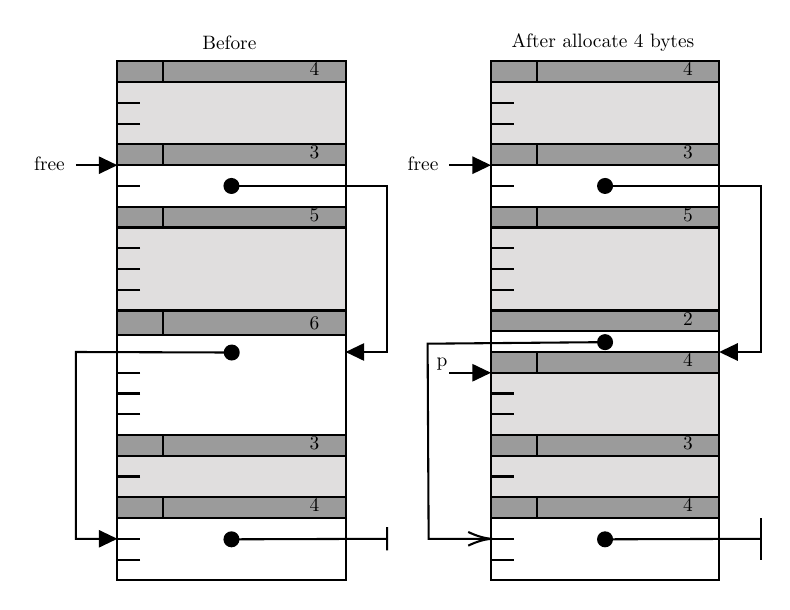
\begin{tikzpicture}[x=0.75pt,y=0.75pt,yscale=-1,xscale=1]
        \draw  [fill={rgb, 255:red, 155; green, 155; blue, 155 }  ,fill opacity=1 ] (100,20) -- (210,20) -- (210,30) -- (100,30) -- cycle ;
        \draw  [fill={rgb, 255:red, 224; green, 222; blue, 222 }  ,fill opacity=1 ] (100,30) -- (210,30) -- (210,60) -- (100,60) -- cycle ;
        \draw    (100,40) -- (111,40) ;
        \draw    (111,50) -- (100,50) ;
        \draw    (122,20) -- (122,30) ;
        \draw  [fill={rgb, 255:red, 155; green, 155; blue, 155 }  ,fill opacity=1 ] (100,60) -- (210,60) -- (210,70) -- (100,70) -- cycle ;
        \draw  [fill={rgb, 255:red, 255; green, 255; blue, 255 }  ,fill opacity=1 ] (100,70) -- (210,70) -- (210,90) -- (100,90) -- cycle ;
        \draw    (100,80) -- (111,80) ;
        \draw    (122,60) -- (122,70) ;
        \draw  [fill={rgb, 255:red, 224; green, 222; blue, 222 }  ,fill opacity=1 ] (100,100) -- (210,100) -- (210,140) -- (100,140) -- cycle ;
        \draw  [fill={rgb, 255:red, 155; green, 155; blue, 155 }  ,fill opacity=1 ] (100,90) -- (210,90) -- (210,100) -- (100,100) -- cycle ;
        \draw    (111,110) -- (100,110) ;
        \draw    (111,120) -- (100,120) ;
        \draw    (111,130) -- (100,130) ;
        \draw    (122,90) -- (122,100) ;
        \draw  [fill={rgb, 255:red, 255; green, 255; blue, 255 }  ,fill opacity=1 ] (100,152) -- (210,152) -- (210,200) -- (100,200) -- cycle ;
        \draw  [fill={rgb, 255:red, 155; green, 155; blue, 155 }  ,fill opacity=1 ] (100,140) -- (210,140) -- (210,152) -- (100,152) -- cycle ;
        \draw    (111,170) -- (100,170) ;
        \draw    (111,180) -- (100,180) ;
        \draw    (122,140) -- (122,152) ;
        \draw    (111,190) -- (100,190) ;
        \draw  [fill={rgb, 255:red, 155; green, 155; blue, 155 }  ,fill opacity=1 ] (100,200) -- (210,200) -- (210,210) -- (100,210) -- cycle ;
        \draw    (122,200) -- (122,210) ;
        \draw  [fill={rgb, 255:red, 224; green, 222; blue, 222 }  ,fill opacity=1 ] (100,210) -- (210,210) -- (210,230) -- (100,230) -- cycle ;
        \draw    (111,220) -- (100,220) ;
        \draw  [fill={rgb, 255:red, 155; green, 155; blue, 155 }  ,fill opacity=1 ] (100,230) -- (210,230) -- (210,240) -- (100,240) -- cycle ;
        \draw  [fill={rgb, 255:red, 255; green, 255; blue, 255 }  ,fill opacity=1 ] (100,240) -- (210,240) -- (210,270) -- (100,270) -- cycle ;
        \draw    (100,250) -- (111,250) ;
        \draw    (111,260) -- (100,260) ;
        \draw    (122,230) -- (122,240) ;
        \draw    (155,80) -- (230,80) -- (230,160) -- (212,160) ;
        \draw [shift={(210,160)}, rotate = 360] [fill={rgb, 255:red, 0; green, 0; blue, 0 }  ][line width=0.75]  [draw opacity=0] (8.93,-4.29) -- (0,0) -- (8.93,4.29) -- cycle    ;
        \draw [shift={(155,80)}, rotate = 0] [color={rgb, 255:red, 0; green, 0; blue, 0 }  ][fill={rgb, 255:red, 0; green, 0; blue, 0 }  ][line width=0.75]      (0, 0) circle [x radius= 3.35, y radius= 3.35]   ;
        \draw    (155.13,160.25) -- (80,160) -- (80,250) -- (98,250) ;
        \draw [shift={(100,250)}, rotate = 180] [fill={rgb, 255:red, 0; green, 0; blue, 0 }  ][line width=0.75]  [draw opacity=0] (8.93,-4.29) -- (0,0) -- (8.93,4.29) -- cycle    ;
        \draw [shift={(155.13,160.25)}, rotate = 180.19] [color={rgb, 255:red, 0; green, 0; blue, 0 }  ][fill={rgb, 255:red, 0; green, 0; blue, 0 }  ][line width=0.75]      (0, 0) circle [x radius= 3.35, y radius= 3.35]   ;
        \draw    (80,70) -- (98,70) ;
        \draw [shift={(100,70)}, rotate = 180] [fill={rgb, 255:red, 0; green, 0; blue, 0 }  ][line width=0.75]  [draw opacity=0] (8.93,-4.29) -- (0,0) -- (8.93,4.29) -- cycle    ;
        \draw    (155,250.25) -- (230,250) ;
        \draw [shift={(230,250)}, rotate = 539.81] [color={rgb, 255:red, 0; green, 0; blue, 0 }  ][line width=0.75]    (0,5.59) -- (0,-5.59)   ;
        \draw [shift={(155,250.25)}, rotate = 359.81] [color={rgb, 255:red, 0; green, 0; blue, 0 }  ][fill={rgb, 255:red, 0; green, 0; blue, 0 }  ][line width=0.75]      (0, 0) circle [x radius= 3.35, y radius= 3.35]   ;
        \draw  [fill={rgb, 255:red, 155; green, 155; blue, 155 }  ,fill opacity=1 ] (280,20) -- (390,20) -- (390,30) -- (280,30) -- cycle ;
        \draw  [fill={rgb, 255:red, 224; green, 222; blue, 222 }  ,fill opacity=1 ] (280,30) -- (390,30) -- (390,60) -- (280,60) -- cycle ;
        \draw    (280,40) -- (291,40) ;
        \draw    (291,50) -- (280,50) ;
        \draw    (302,20) -- (302,30) ;
        \draw  [fill={rgb, 255:red, 155; green, 155; blue, 155 }  ,fill opacity=1 ] (280,60) -- (390,60) -- (390,70) -- (280,70) -- cycle ;
        \draw  [fill={rgb, 255:red, 255; green, 255; blue, 255 }  ,fill opacity=1 ] (280,70) -- (390,70) -- (390,90) -- (280,90) -- cycle ;
        \draw    (280,80) -- (291,80) ;
        \draw    (302,60) -- (302,70) ;
        \draw  [fill={rgb, 255:red, 224; green, 222; blue, 222 }  ,fill opacity=1 ] (280,100) -- (390,100) -- (390,140) -- (280,140) -- cycle ;
        \draw  [fill={rgb, 255:red, 155; green, 155; blue, 155 }  ,fill opacity=1 ] (280,90) -- (390,90) -- (390,100) -- (280,100) -- cycle ;
        \draw    (291,110) -- (280,110) ;
        \draw    (291,120) -- (280,120) ;
        \draw    (291,130) -- (280,130) ;
        \draw    (302,90) -- (302,100) ;
        \draw  [fill={rgb, 255:red, 255; green, 255; blue, 255 }  ,fill opacity=1 ] (280,150) -- (390,150) -- (390,200) -- (280,200) -- cycle ;
        \draw  [fill={rgb, 255:red, 155; green, 155; blue, 155 }  ,fill opacity=1 ] (280,140) -- (390,140) -- (390,150) -- (280,150) -- cycle ;
        \draw  [fill={rgb, 255:red, 155; green, 155; blue, 155 }  ,fill opacity=1 ] (280,200) -- (390,200) -- (390,210) -- (280,210) -- cycle ;
        \draw    (302,200) -- (302,210) ;
        \draw  [fill={rgb, 255:red, 224; green, 222; blue, 222 }  ,fill opacity=1 ] (280,210) -- (390,210) -- (390,230) -- (280,230) -- cycle ;
        \draw    (291,220) -- (280,220) ;
        \draw  [fill={rgb, 255:red, 155; green, 155; blue, 155 }  ,fill opacity=1 ] (280,230) -- (390,230) -- (390,240) -- (280,240) -- cycle ;
        \draw  [fill={rgb, 255:red, 255; green, 255; blue, 255 }  ,fill opacity=1 ] (280,240) -- (390,240) -- (390,270) -- (280,270) -- cycle ;
        \draw    (280,250) -- (291,250) ;
        \draw    (291,260) -- (280,260) ;
        \draw    (302,230) -- (302,240) ;
        \draw    (335,80) -- (410,80) -- (410,160) -- (392,160) ;
        \draw [shift={(390,160)}, rotate = 360] [fill={rgb, 255:red, 0; green, 0; blue, 0 }  ][line width=0.75]  [draw opacity=0] (8.93,-4.29) -- (0,0) -- (8.93,4.29) -- cycle    ;
        \draw [shift={(335,80)}, rotate = 0] [color={rgb, 255:red, 0; green, 0; blue, 0 }  ][fill={rgb, 255:red, 0; green, 0; blue, 0 }  ][line width=0.75]      (0, 0) circle [x radius= 3.35, y radius= 3.35]   ;
        \draw    (260,70) -- (278,70) ;
        \draw [shift={(280,70)}, rotate = 180] [fill={rgb, 255:red, 0; green, 0; blue, 0 }  ][line width=0.75]  [draw opacity=0] (8.93,-4.29) -- (0,0) -- (8.93,4.29) -- cycle    ;
        \draw    (335,250.25) -- (410,250) ;
        \draw [shift={(335,250.25)}, rotate = 359.81] [color={rgb, 255:red, 0; green, 0; blue, 0 }  ][fill={rgb, 255:red, 0; green, 0; blue, 0 }  ][line width=0.75]      (0, 0) circle [x radius= 3.35, y radius= 3.35]   ;
        \draw    (410,240) -- (410,260) ;
        \draw  [fill={rgb, 255:red, 155; green, 155; blue, 155 }  ,fill opacity=1 ] (280,160) -- (390,160) -- (390,170) -- (280,170) -- cycle ;
        \draw  [fill={rgb, 255:red, 224; green, 222; blue, 222 }  ,fill opacity=1 ] (280,170) -- (390,170) -- (390,200) -- (280,200) -- cycle ;
        \draw    (280,180) -- (291,180) ; 
        \draw    (291,190) -- (280,190) ;
        \draw    (302,160) -- (302,170) ; 
        \draw    (260,170) -- (278,170) ;
        \draw [shift={(280,170)}, rotate = 180] [fill={rgb, 255:red, 0; green, 0; blue, 0 }  ][line width=0.75]  [draw opacity=0] (8.93,-4.29) -- (0,0) -- (8.93,4.29) -- cycle    ;
        \draw    (335,155.25) -- (249.5,156) -- (250,250) -- (278,250) ;
        \draw [shift={(280,250)}, rotate = 180] [color={rgb, 255:red, 0; green, 0; blue, 0 }  ][line width=0.75]    (10.93,-3.29) .. controls (6.95,-1.4) and (3.31,-0.3) .. (0,0) .. controls (3.31,0.3) and (6.95,1.4) .. (10.93,3.29)   ;
        \draw [shift={(335,155.25)}, rotate = 179.5] [color={rgb, 255:red, 0; green, 0; blue, 0 }  ][fill={rgb, 255:red, 0; green, 0; blue, 0 }  ][line width=0.75]      (0, 0) circle [x radius= 3.35, y radius= 3.35]   ;
        \draw (195,24) node [scale=0.7] [align=left] {4};
        \draw (195,64) node [scale=0.7] [align=left] {3};
        \draw (195,94) node [scale=0.7] [align=left] {5};
        \draw (195,146) node [scale=0.7] [align=left] {6};
        \draw (195,204) node [scale=0.7] [align=left] {3};
        \draw (195,234) node [scale=0.7] [align=left] {4};
        \draw (67.33,69.33) node [scale=0.7] [align=left] {free};
        \draw (375,24) node [scale=0.7] [align=left] {4};
        \draw (375,64) node [scale=0.7] [align=left] {3};
        \draw (375,94) node [scale=0.7] [align=left] {5};
        \draw (375,144) node [scale=0.7] [align=left] {2};
        \draw (375,204) node [scale=0.7] [align=left] {3};
        \draw (375,234) node [scale=0.7] [align=left] {4};
        \draw (247.33,69.33) node [scale=0.7] [align=left] {free};
        \draw (375,164) node [scale=0.7] [align=left] {4};
        \draw (256.5,166) node [scale=0.7] [align=left] {p};
        \draw (154,11) node [scale=0.7] [align=left] {Before};
        \draw (334,11) node [scale=0.7] [align=left] {After allocate 4 bytes};
    \end{tikzpicture}
    \caption{First-fit allocation policy}
    \label{fig:memman}
\end{figure}

\begin{tcolorbox}
\ArrowBoldDownRight \textit{Note}: Because memory is statically declared, it will make the application appear to consume a lot of RAM, even before any memory has been allocated from it.
\end{tcolorbox}

\begin{tcolorbox}
\AsteriskBold \textit{Warning}: All the memory management APIs are NOT interrupt-safe. Use these APIs only from the base context.
\end{tcolorbox}

\begin{tcolorbox}
\AsteriskBold \textit{Warning}: The application is not exempt from memory leaks if the user does not perform adequate memory management. Here, the worst case scenario can occur in the absence of free memory. 
\end{tcolorbox}

\subsubsection{Memory pools}

A memory pool its a special resource that allows memory blocks to be dynamically allocated from a user-designated memory region. Instead of typical pools with fixed-size block allocation, the pools in QuarkTS can be of any size, thereby the user is responsible for selecting the appropriate memory pool to allocate data with the same size. 

The \textit{default} memory management unit resides in a memory pool object. Also called the \textit{default pool}. The total amount of available heap space in the default memory pool is set by \lstinline{Q_DEFAULT_HEAP_SIZE}, which is defined in \lstinline{qconfig.h}.

Besides the \textit{default} pool, any number of additional memory pools can be defined. Like any other object in QuarkTS, memory pools are referenced by handles, a variable of type \lstinline{qMemMang_Pool_t} \index{\lstinline{qMemMang_Pool_t}} and should be initialized before use with the \lstinline{qMemMang_Pool_Setup()} \index{\lstinline{qMemMang_Pool_Setup}} API function.
\medskip

\begin{lstlisting}[style=CStyle]
qBool_t qMemMang_Pool_Setup( qMemMang_Pool_t * const mPool, void* Area, 
                             size_t size )
\end{lstlisting}

\subsubsection*{Parameters}
\begin{itemize}
    \item \lstinline{mPool} : A pointer to the memory pool instance. 
    \item \lstinline{Area} :  A pointer to a memory region (\lstinline{qUINT8_t}) statically allocated to act as Heap of the memory pool. The size of this block should match the \lstinline{size} argument.
    \item \lstinline{size} : The size of the memory block pointed by \lstinline{Area}. 
\end{itemize}

To perform operations in another memory pool, besides the \textit{default} pool, an explicit switch should be performed using \lstinline{qMemMang_Pool_Select()} \index{\lstinline{qMemMang_Pool_Select}}. Here, a pointer to the target pool should be passed as input argument.  From now on, every call to \lstinline{qMalloc()}, or \lstinline{qFree()} will run over the newly selected memory pool. To return to  the \textit{default pool},  a new call to  \lstinline{qMemMang_Pool_Select()} is required passing \lstinline{NULL} as input argument. 
\medskip

\begin{lstlisting}[style=CStyle]
void qMemMang_Pool_Select( qMemMang_Pool_t * const mPool )
\end{lstlisting}

To keep track of the memory usage, the \lstinline{qMemMang_Get_FreeSize()} \index{\lstinline{qMemMang_Get_FreeSize}} API function returns the number of free bytes in the memory pool at the time the function is called.
\medskip

\begin{lstlisting}[style=CStyle]
size_t qMemMang_Get_FreeSize( void )
\end{lstlisting}

\subsubsection*{Usage example:}

\lstinputlisting[style=CStyle]{sec3memmangdem1.c}

\subsection{Trace and debugging}
QuarkTS include some basic macros to print out debugging messages. Messages can be simple text or the value of variables in specific base-formats. 
To use the trace macros, a single-char output function must be defined using the \lstinline{qTrace_Set_OutputFcn()} macro.\index{\lstinline{qTrace_Set_OutputFcn}}
\medskip

\begin{lstlisting}[style=CStyle]
qTrace_Set_OutputFcn( qPutChar_t fcn )
\end{lstlisting}

Where \lstinline{fcn} is a pointer to the single-char output function following the prototype:
\medskip

\begin{lstlisting}[style=CStyle]
void SingleChar_OutputFcn( void *sp, const char c ){
    /*
    TODO : print out the c variable using the
    selected peripheral.
    */
}
\end{lstlisting}

The body of this user-defined function should have a hardware-dependent code to print out the \lstinline{c} variable through a specific peripheral.

\subsubsection{Viewing variables}
For viewing or tracing a variable (up to 32-bit data) through debug, one of the following macros are available:
\index{\lstinline{qTrace_Var}} \index{\lstinline{qTrace_Variable}} \index{\lstinline{qDebug_Var}} \index{\lstinline{qDebug_Variable}}
\medskip

\begin{lstlisting}[style=CStyle]
qTrace_Var( Var, DISP_TYPE_MODE )
qTrace_Variable( Var, DISP_TYPE_MODE )
\end{lstlisting}
\begin{lstlisting}[style=CStyle]
qDebug_Var( Var, DISP_TYPE_MODE )
qDebug_Variable( Var, DISP_TYPE_MODE )
\end{lstlisting}

\subsubsection*{Parameters:}
\begin{itemize}
    \item \lstinline{Var} : The target variable. 
    \item \lstinline{DISP_TYPE_MODE } :  Visualization mode. It must be one of the following parameters(case sensitive): \lstinline{Bool}, \lstinline{Float}, \lstinline{Binary}, \lstinline{Octal}, \lstinline{Decimal}, \lstinline{Hexadecimal}, \lstinline{UnsignedBinary}, \lstinline{UnsignedOctal}, \lstinline{UnsignedDecimal}, \lstinline{UnsignedHexadecimal}. 
\end{itemize}

The only difference between \lstinline{qTrace_} and  \lstinline{Debug}, is that \lstinline{qTrace_} macros, print out additional information provided by the \lstinline{__FILE__}, \lstinline{__LINE__} and \lstinline{__func__} built-in preprocessing macros, mostly available in common C compilers. 

\subsubsection{Viewing a memory block}
For tracing memory from a specified target address, one of the following macros are available: \index{\lstinline{qTrace_Mem}} \index{\lstinline{qTrace_Memory}}

\begin{lstlisting}[style=CStyle]
qTrace_Mem( Pointer, BlockSize )
qTrace_Memory( Pointer, BlockSize )
\end{lstlisting}

\subsubsection*{Parameters:}
\begin{itemize}
    \item \lstinline{Pointer} : The target memory address.
    \item \lstinline{Size} : Number of bytes to be visualized.
\end{itemize}

Hexadecimal notation it's used to format the output of these macros.

\subsubsection{Usage}

In the example below, an UART output function is coded to act as the printer. Here, the target MCU is an ARM-Cortex M0 with the UART1 as the selected peripheral for this purpose.
\medskip

\begin{lstlisting}[style=CStyle]
void putUART1( void *sp, const char c ){
    /* hardware specific code */
    UART1_D = c;
    while ( !(UART1_S1 & UART_S1_TC_MASK) ) {} /*wait until TX is done*/ 
}
\end{lstlisting}  

As seen above, the function follows the required prototype. Later, in the main thread, a call to the \lstinline{qSetDebugFcn()} is used to set up the output-function.

\begin{lstlisting}[style=CStyle]
int main( void ){
   qTrace_Set_OutputFcn( putUART1 );
   ... 
   ...
}
\end{lstlisting}  

After that, trace macros will be available for use.

\begin{lstlisting}[style=CStyle]
void IO_TASK_Callback( qEvent_t e ){
   static qUINT32_t Counter = 0;
   float Sample;
   ...
   ... 
   qTrace_Message( "IO TASK running..." );
   Counter++;
   qTrace_Variable( Counter, UnsignedDecimal );
   Sample = SensorGetSample();
   qTrace_Variable( Sample, Float );
   ...
   ...
}
\end{lstlisting}

\newpage